\chapter{Results}

As proposed in the objectives, the most important results on the analysis of
the ELF, $\rho$ and NCI in water clusters are shown in this chapter.

\section{Systems}

All systems used in this work were taken from the literature
\cite{Temelso2011}. In particular, there are divided in 3 groups of systems.
Set 1 contains global minimal clusters, increasing the number of water
molecules (from dimer to pentamer) and a pentamer that is a local minimum. Set
2 contains several dimers with different configurations. Set 3 contains
different local minima from dimer to hexamer. All systems are plotted in the
Figures \ref{Set1}, \ref{Set2} and \ref{Set3}, the three sets mentioned above.

The first group was used as the assessment group for computational processing,
choosing the best parameters and methods of integration (topic discussed in
Section \ref{SecTheory}). Once all calculations were completed with good
accuracy for Set 1, we started to compute Sets 2 and 3 with the help of some
scripts (Supporting Information \ref{SIscript}).

\newpage

\begin{figure}[!hp]
  \centering
  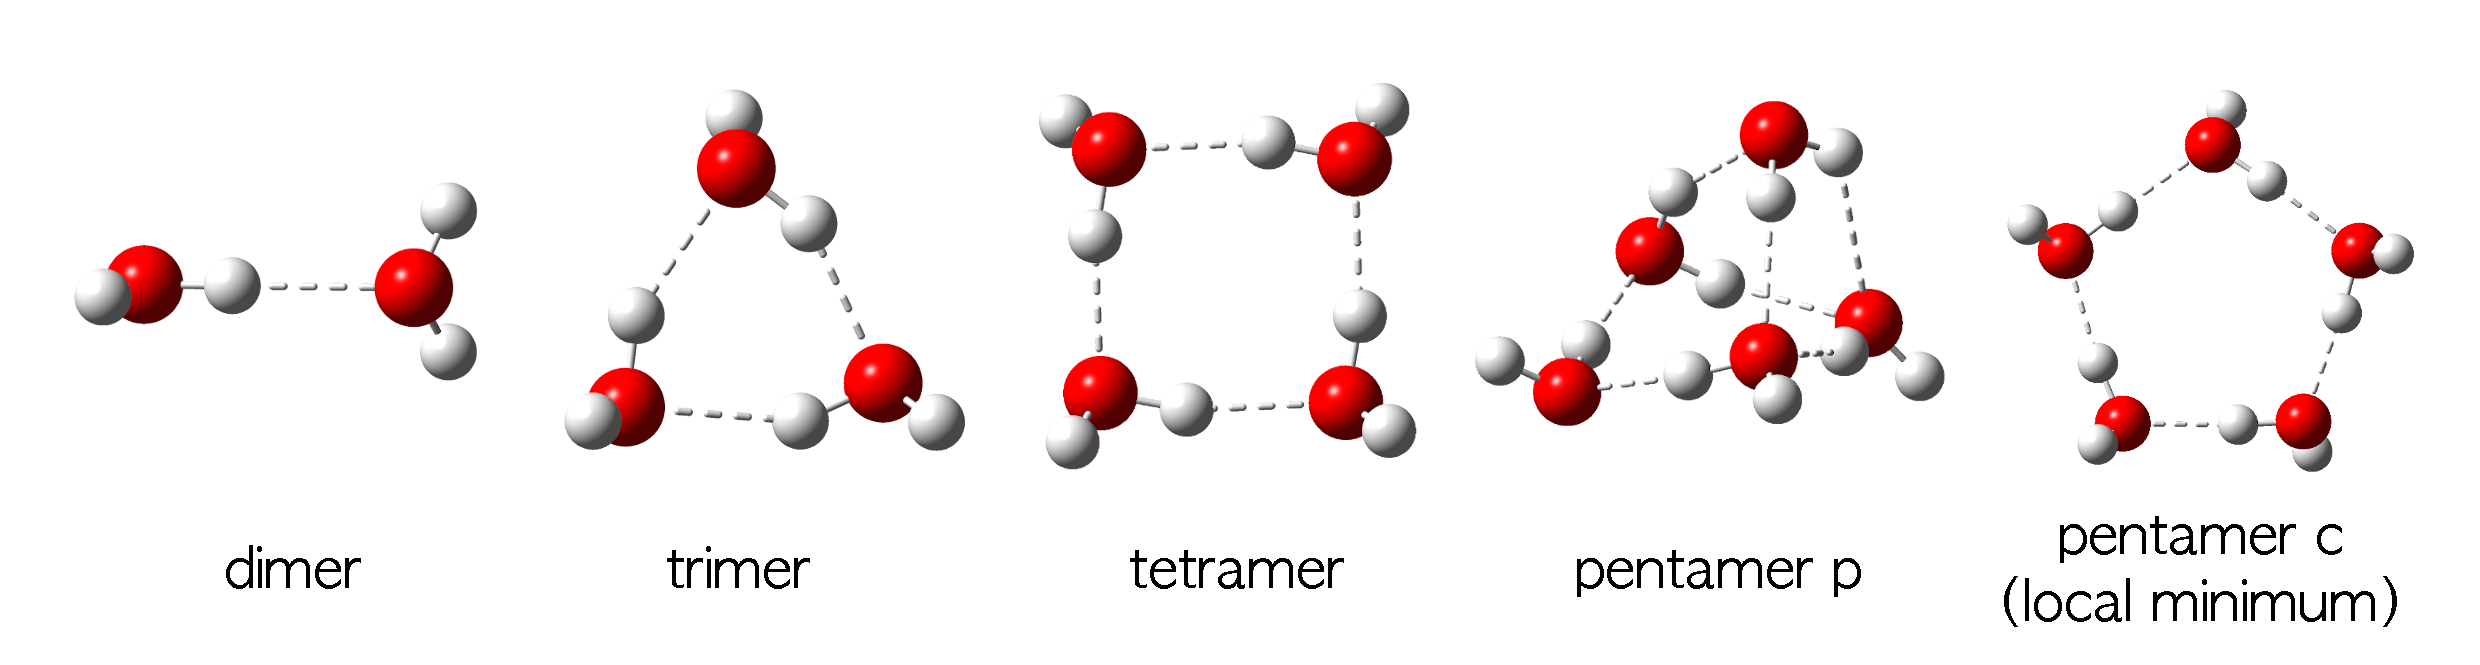
\includegraphics[width=1\textwidth]{4/plots/dibujitos/set1}
  \caption{Set 1 of water clusters (global minima).}
  \label{Set1}
\end{figure}
\begin{figure}[!hp]
  \centering
  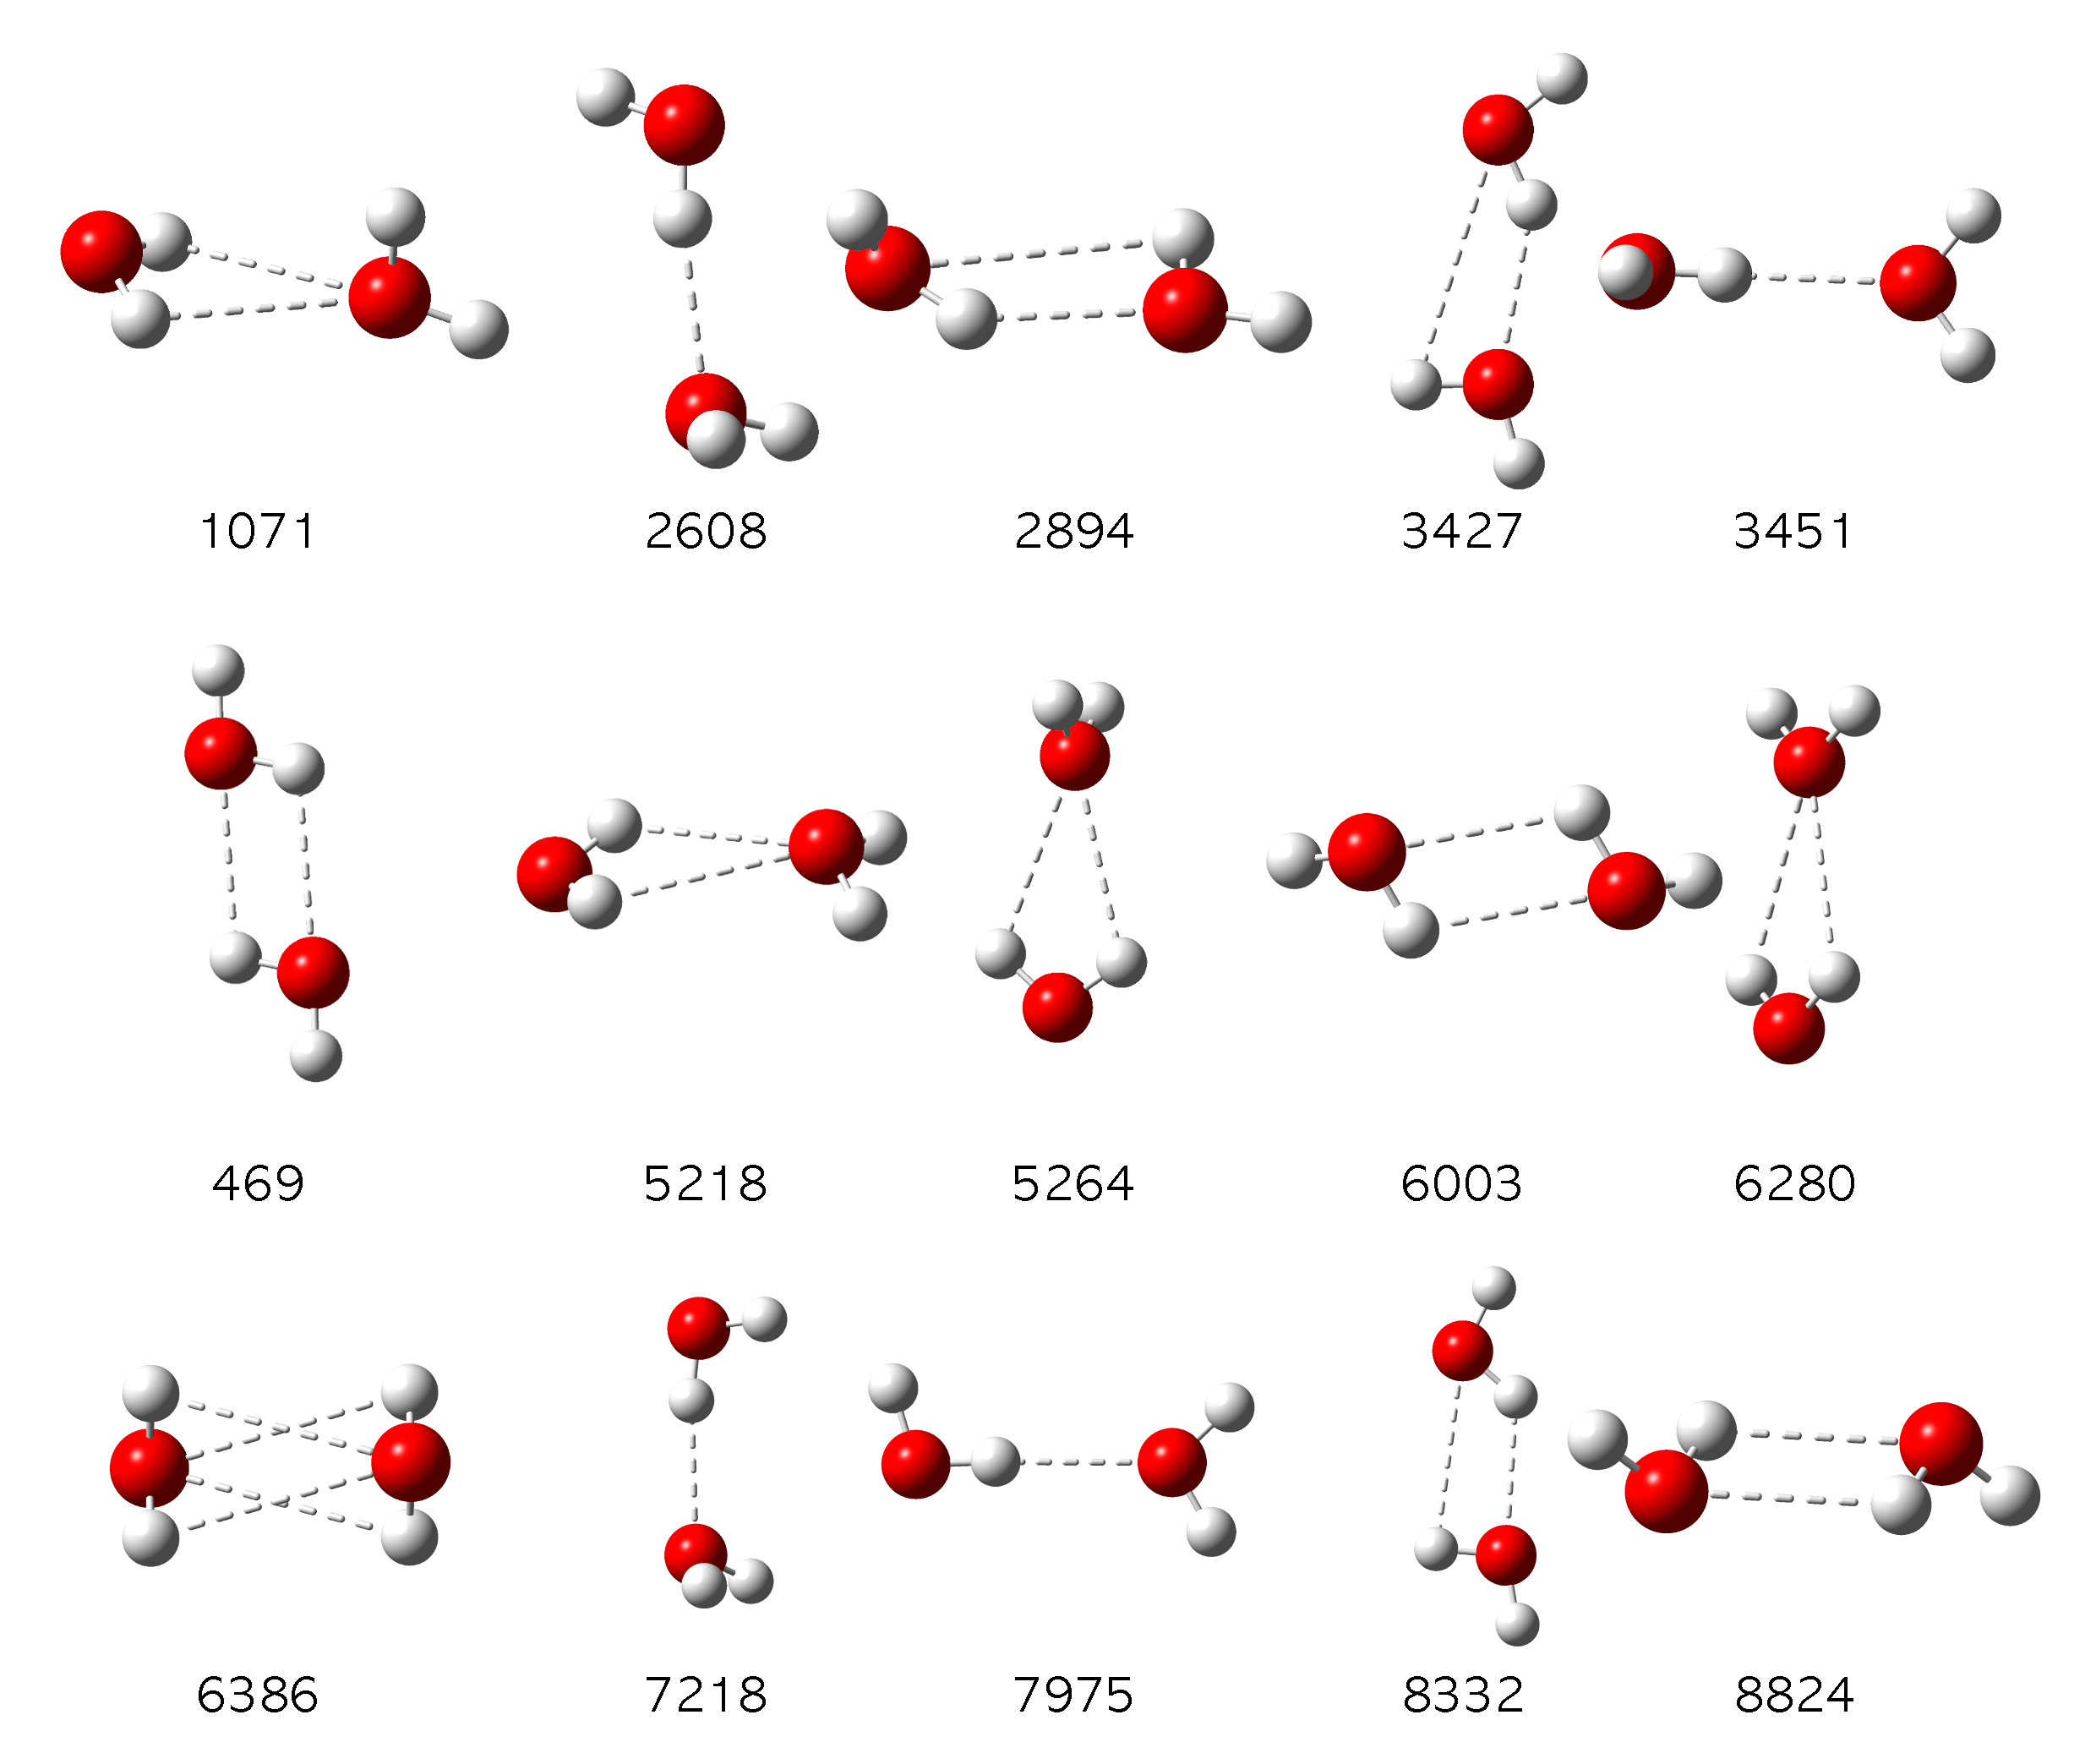
\includegraphics[width=1\textwidth]{4/plots/dibujitos/set2}
  \caption{Set 2 of water clusters. Local minima of dimer clusters. Clusters
  are named by the file name where the coordinates were taken.}
  \label{Set2}
\end{figure}
\begin{figure}[h!p]
  \centering
  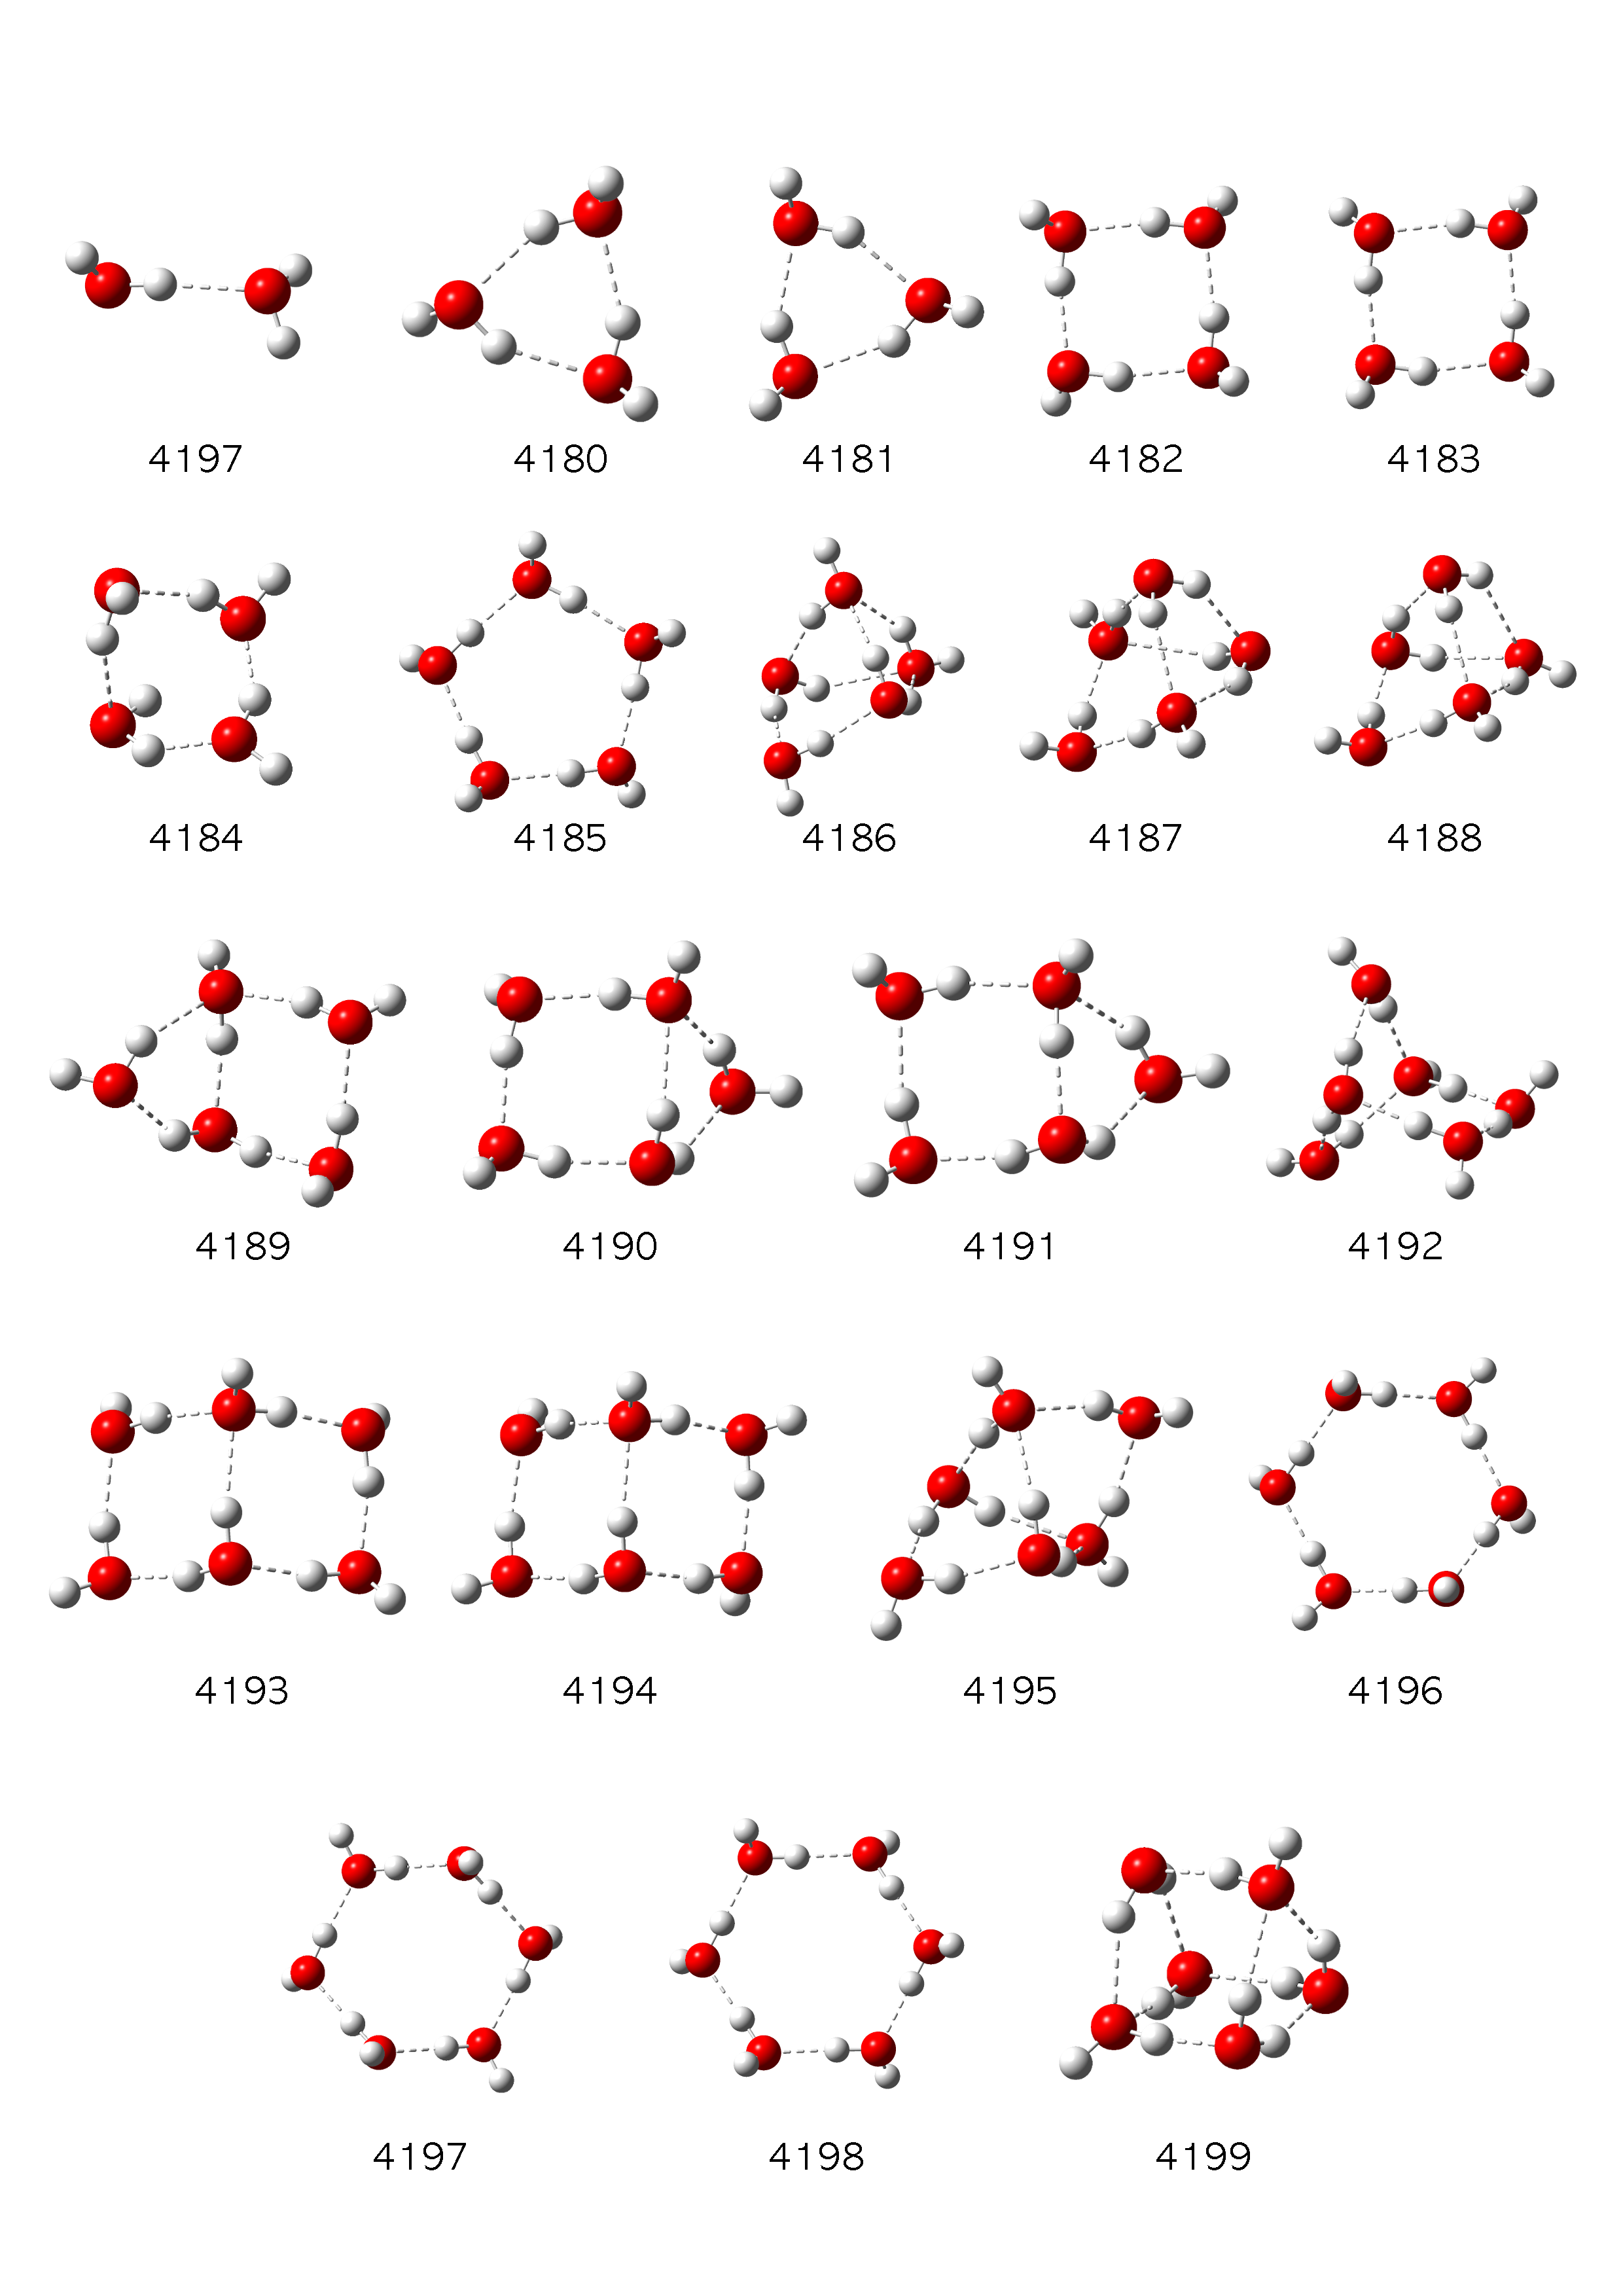
\includegraphics[width=1\textwidth]{4/plots/dibujitos/set3}
  \caption{Set 3 of water clusters. Local minima taken from \citet{Temelso2011}.
  Clusters are named by the file name where the coordinates were taken.}
  \label{Set3}
\end{figure}

\newpage

\section{Theory level, method election}\label{SecTheory}

The choice of the M06-2X/6-311++G(d,p) theory level is justified by the
combination of the exchange-correlation functional with triple-zeta quality
basis sets which adequately reproduce the cooperative and anti-cooperative
behavior.  This methodology allows an accurate description at a moderate
computational cost, as shown in the work of Jiménez Gravalos et al
\citenum{JimenezGravalos2019}.

\begin{figure}[htb]
    \begin{minipage}[t]{0.48\textwidth}
      \centering
      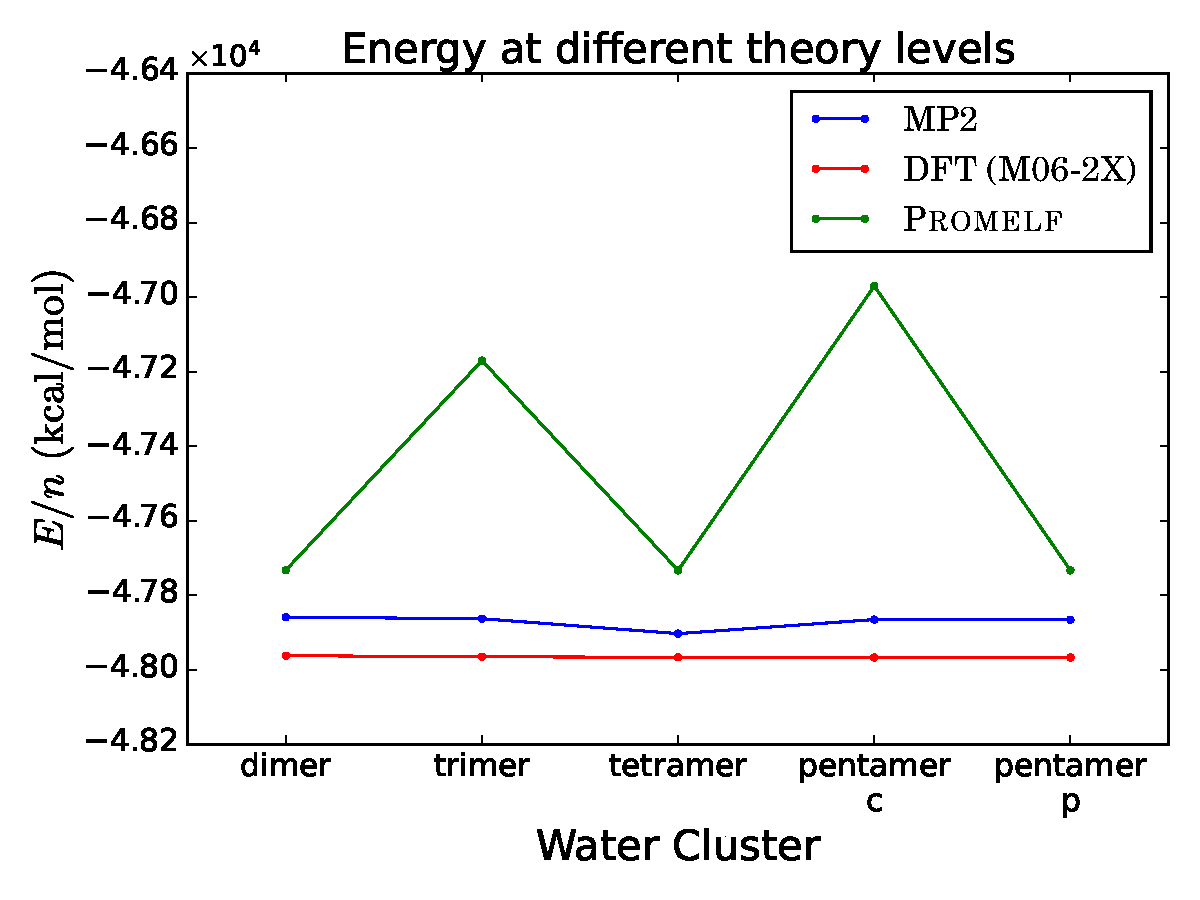
\includegraphics[width=1.01\linewidth]{4/plots/theory_level/mp2dftpromelf.pdf}
      \caption{Energy divided by the cluster size in \gls{MP2}, DFT and {\sc{Promelf}}, Set 1.}
      \label{mp2vsm062x}
    \end{minipage}%
    \hfill
    \begin{minipage}[t]{0.48\textwidth}
      \centering
      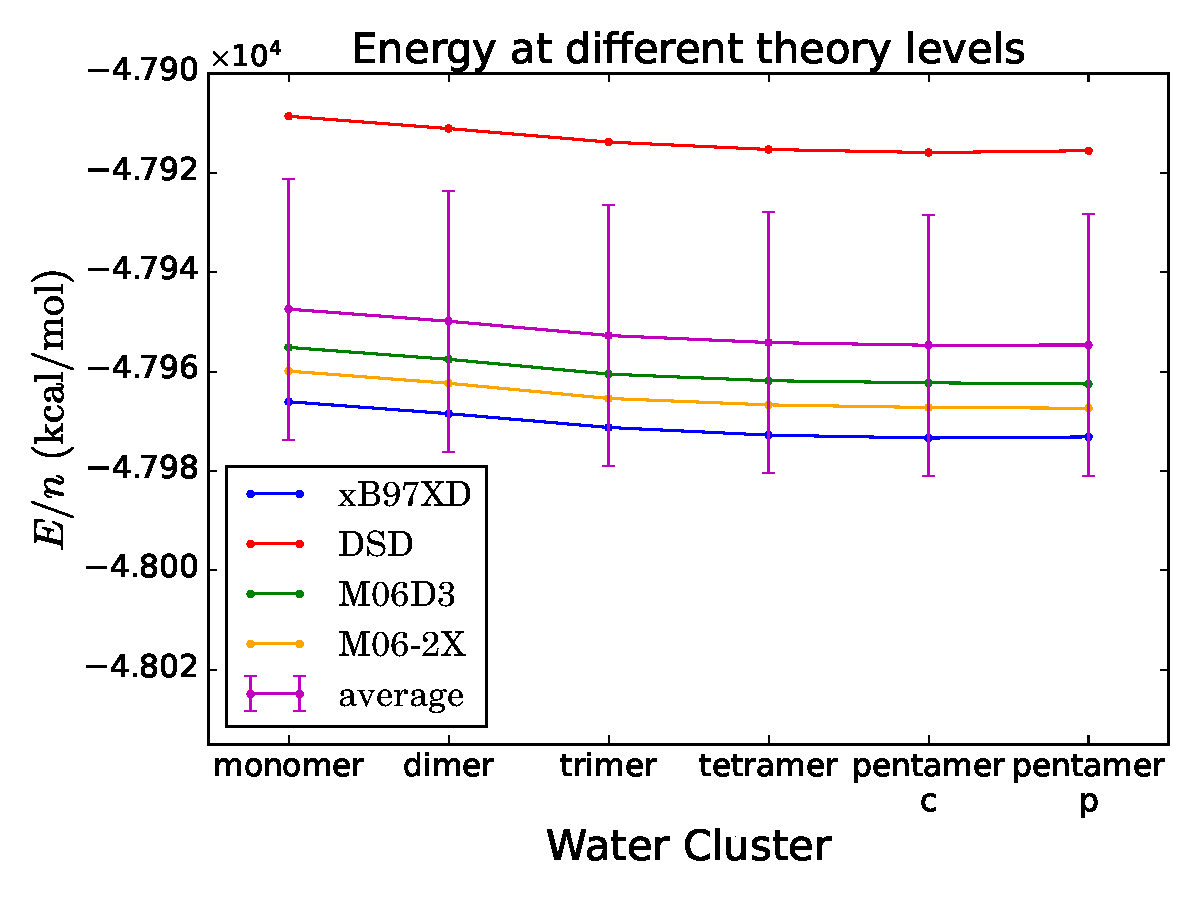
\includegraphics[width=1.01\linewidth]{4/plots/theory_level/functionals.pdf}
      \caption{Energy divided by the cluster size in wB97XD, DSD, M06-2X and M06D3 functionals.}
      \label{energies}
    \end{minipage}%
\end{figure}
\begin{wrapfigure}[10]{r}{0.48\textwidth} %this figure will be at the right
    \centering
\vspace*{-1cm}
    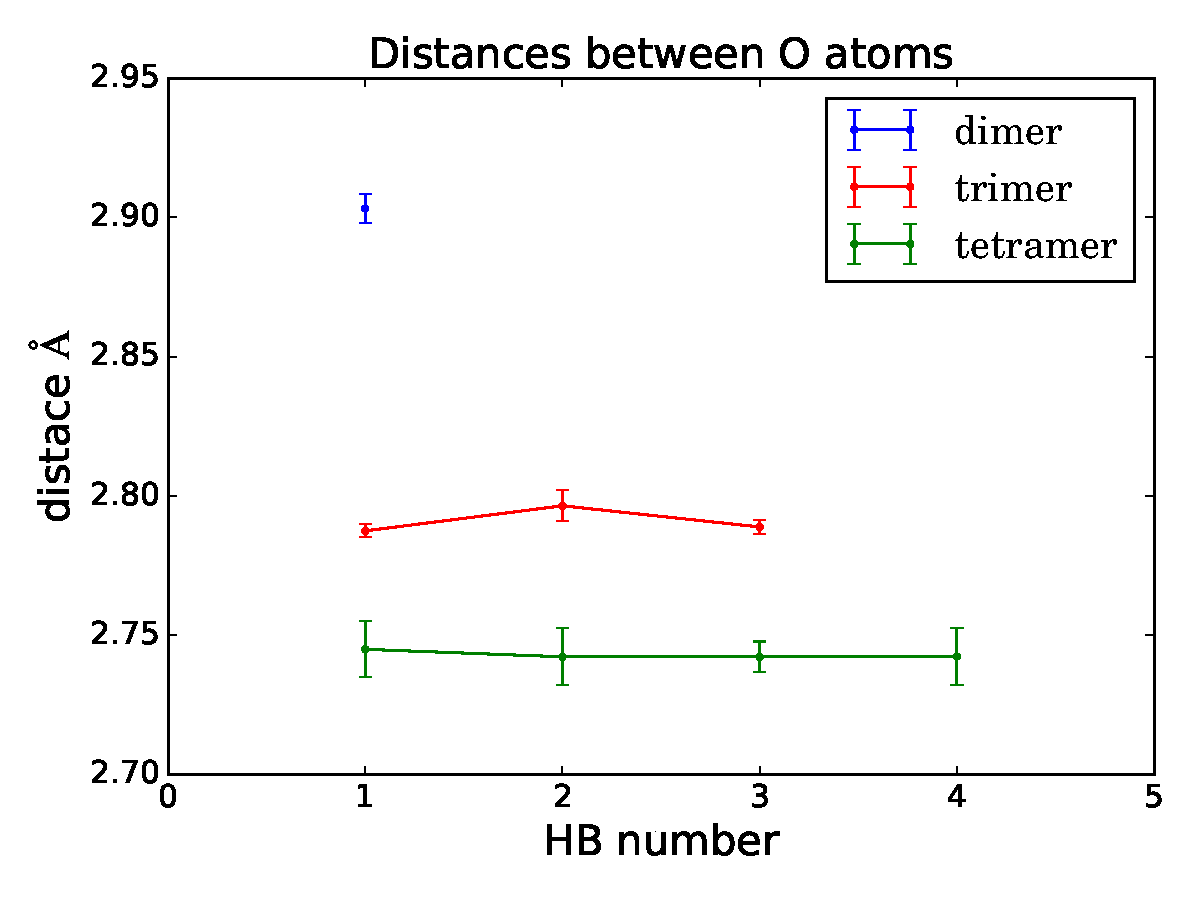
\includegraphics[width=0.5\textwidth]{4/plots/theory_level/distances.pdf}
    \caption{Distances between water molecules taking the oxygen atoms as a reference.}
    \label{distances}
\end{wrapfigure}

We also tried an \textit{ab initio} method, Møller–Plesset at second order,
getting good results for the energy, but having numerical problems with the
{\sc{Promelf}} program (problems that will be described later on). Then the use
of a DFT method was thought as a good solution, minimizing most of the
numerical issues with {\sc{Promelf}} and also providing similar values for the
energy, as we can see in the Figure \ref{mp2vsm062x}, where even if the energy
variation is bigger for {\sc{Promelf}} vs DFT than the difference between MP2
and DFT, the variation per water molecule is still in the same magnitude order.

\newpage
%\pagebreak

Once we known that we would use DFT, we also decided to compare different
functionals, analyzing not only the energy at the same geometry, but also doing
a geometry optimization at each level, looking at how the distances change.
See Figures \ref{energies} and \ref{distances}, where in case of the energies
the differences are around tens of \si{\kilo\calorie\per\mole}, and no any
oxygen-oxygen distance change enough large to lend ambiguity between the
different cases of \gls{n-mer}\footnote{$n$-mer = aggregate of $n$ molecules.}
distances.

Later one, when M062X was chosen as the functional that we would use, we did a
systematic analysis of the basis set dependency, through variations within
Truhlar’s calendar \cite{Papajak2011} we had an idea of the basis set
dependency (see Figure \ref{calendar_limit}). Particularly, the numerical value
of the correlation energy limit is computable as plotted in Figure
\ref{limit_MP2}. In both previous figures we can see that the energy values do
not change significantly after the use of aug-pVTZ, the above added to the fact
that using a quadruple zeta basis set increase significantly the computing
time.  These observations, together with the previous assessment carried out by
Jiménez Gravalos et al \citenum{JimenezGravalos2019}, justify our selection of
the M06-2X/aug-cc-pVTZ level of theory. 

\begin{figure}[h]
    \begin{minipage}[t]{0.48\textwidth}
      \centering
      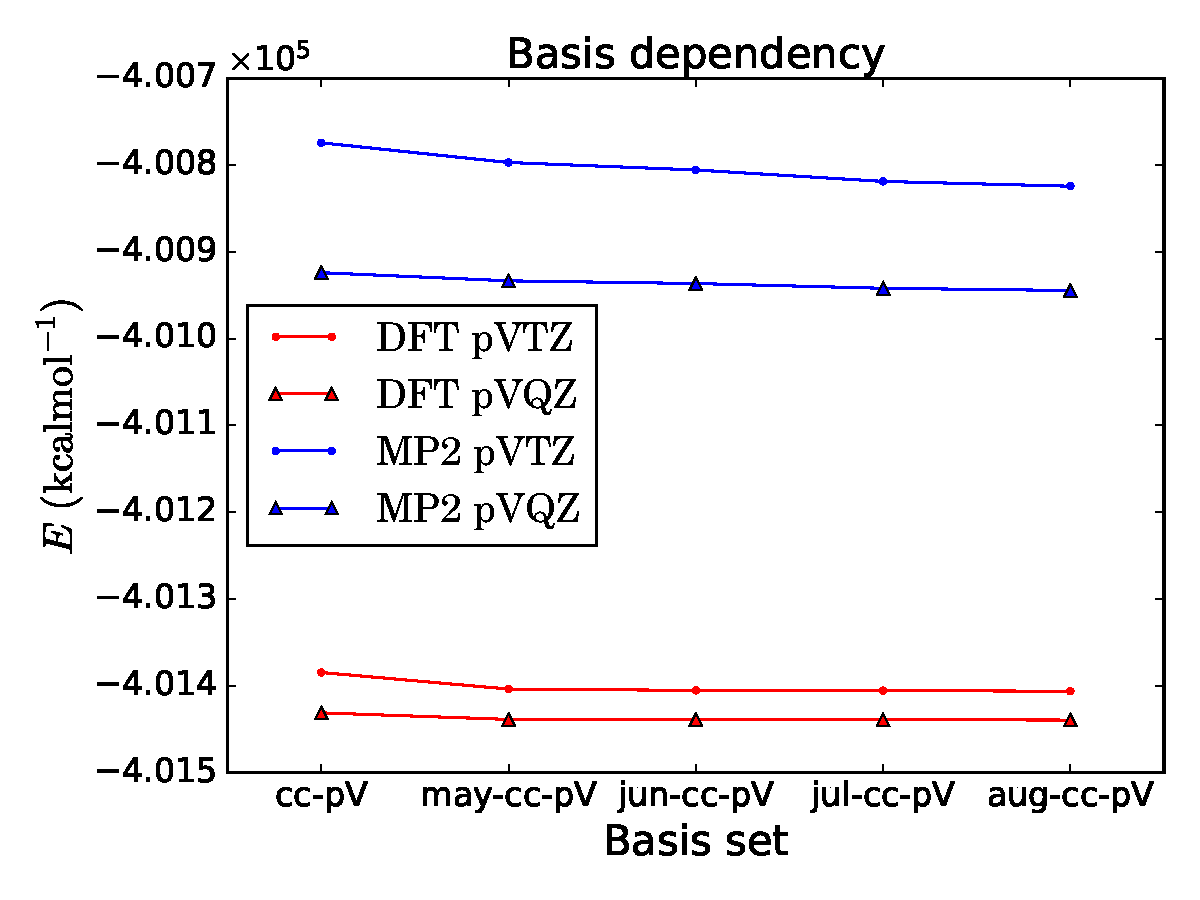
\includegraphics[width=\textwidth]{4/plots/basis/dimer_basis.pdf}
      \caption{Energy in different basis set in water dimer system.}
      \label{calendar_limit}
    \end{minipage}%
    \hfill
    \begin{minipage}[t]{0.48\textwidth}
      \centering
      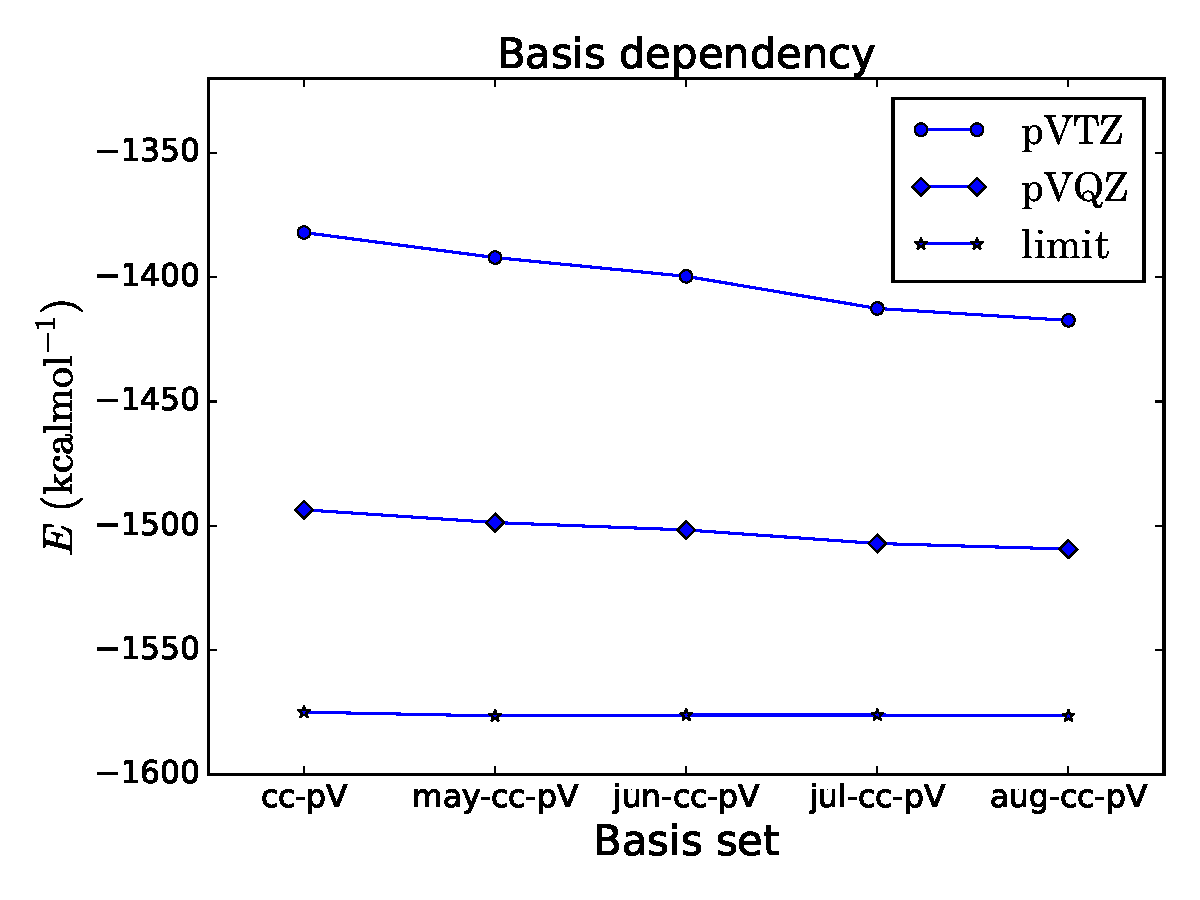
\includegraphics[width=1\textwidth]{4/plots/basis/limit_basis.pdf}
      \caption{Limit for $E_{corr}$ in water dimer system.}
      \label{limit_MP2}
    \end{minipage}%
\end{figure}

The wavefunctions obtained at the M06-2X/aug-cc-pVTZ level were analyzed by
means of ELF thanks to the {\sc{Promelf}} program.  However, some numerical
problems appeared: $i$) the energy showed a considerable difference between the
one obtained with {\sc{Gaussian16}} and the {\sc{Promelf}} output (around 8
$\mathrm{E_h}$), $ii$) the charge sum of all centers was not equal to the
molecule charge value (zero in those cases), where {\sc{Promelf}} gave around 5
atomic units of charge in worst cases.

Those were the reasons why we guessed that the problems came from the numerical
integration method and its accuracy, particularly with the solid angle grid.
Because, if a numerical value is affected by $i$) the solid angle $ii$) the
radial coordinate, and those values are (numerically, computationally) zero,
the whole \texttt{DO for loop} that computes the integral is summing zero in
all steps.

We tried many different setups for the calculation.  Fortunately, the problems
were fixed by modifying:
$i$)
the radial coordinate, that specifies the largest value of the radial
coordinate in the integration, by default is 10.0, and we changed it to 6.0;
$ii$)
the default value used for points in the radial grid outside B-spheres is 100,
we changed to 512;
$iii$)
the way to define the mapping function $ r(u) $ $( -1 \leqslant u \leqslant +1
)$ outside the B-spheres, the way we use is $ r(u) = r_b \frac{1+u}{1 - u
+\eta} + r_0 $ where $r_b$ is a measure of the atomic radius (these radii are
taken as the Slater-Bragg radii).

All these alterations of the default values were already available in the code.
We also did attempts modifying the radial quadrature used in the integration
within the B-spheres. However, the trapezoidal method (the easiest one), with
the previous changes gives similar values than those given by more
sophisticated methods, with the advantage that the trapezoidal method is the
cheapest method in computational time.


\section{Electronic Localization Function Analysis}

\begin{wrapfigure}[9]{r}{0.3\textwidth} %this figure will be at the right
    \centering
    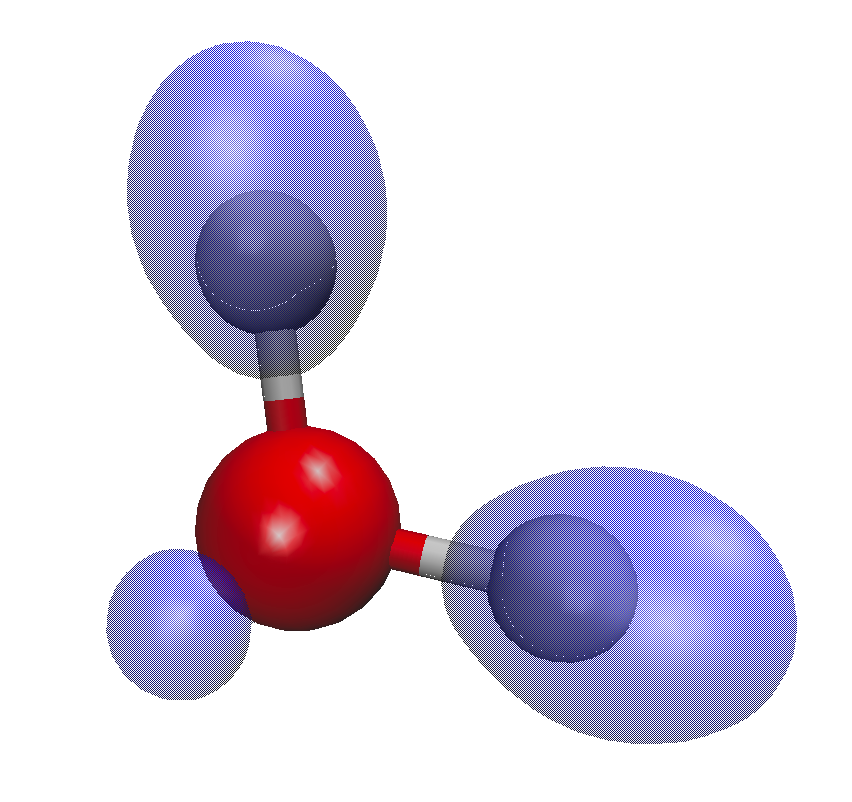
\includegraphics[width=0.3\textwidth]{4/plots/elf/new/waterELF.png}
    \caption{ELF in water molecule (isovalue = 0.9).}
    \label{awa}
\end{wrapfigure}

The first two systems computed to know how the ELF behaves in water clusters
were the water molecule and the dimer, that because in the first one we have
the isolated molecule and in the second one the system has only one acceptor
and one donor, where each molecule has no other interaction(s). Thus, they
constituted good references.

All plots were made using the same isosurface value for all systems in this
section, isovalue = 0.9. Thus, we can compare the systems just by mere visual
plot inspection.

In the Figure \ref{awa} we can see how the basins have the same volume for a
given ELF value for both H atoms, and also for lone electron pairs. Then, one
of the easiest things to see in the water dimer (Figure \ref{dimer}) is how the
ELF changes in the H atoms and in the lone pairs, since the chemical situation
changes for those ELF maxima.

\begin{wrapfigure}{l}{0.4\textwidth}
  \centering
  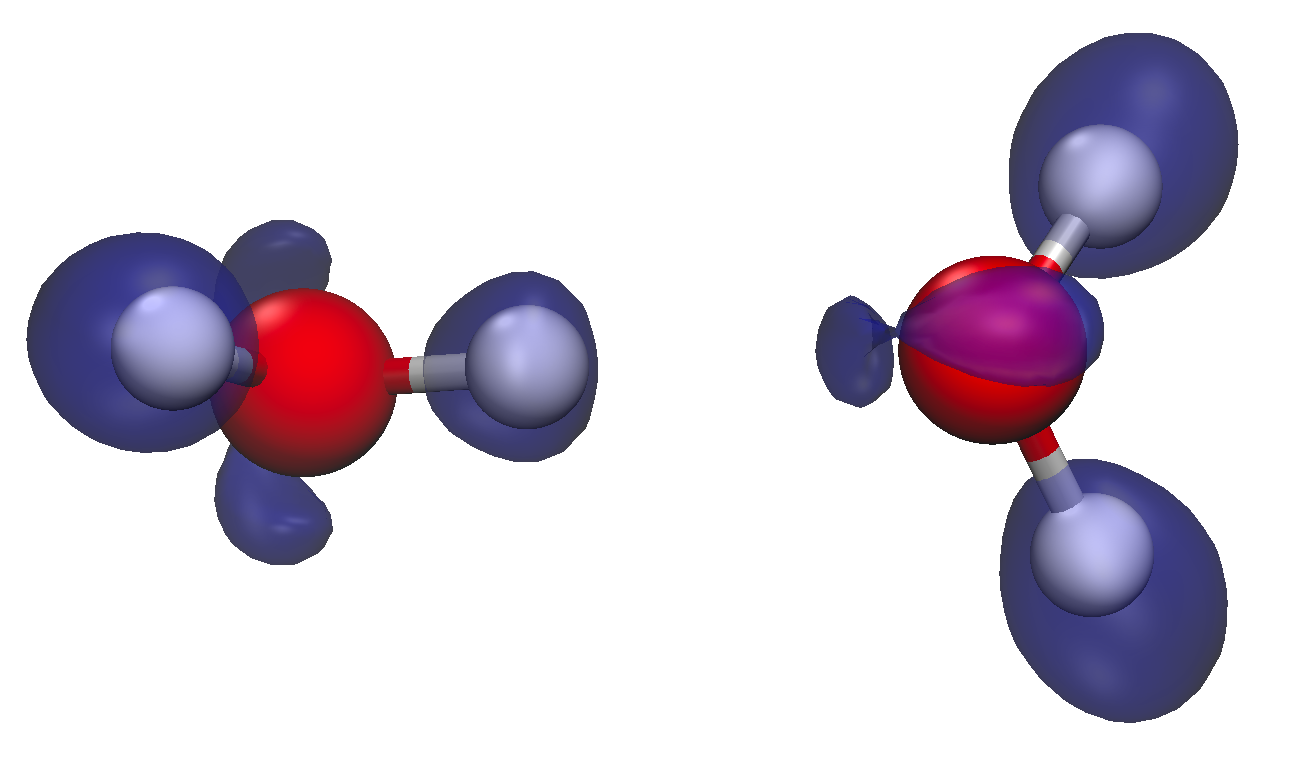
\includegraphics[width=0.4\textwidth]{4/plots/elf/new/dimerELF.png}
  \caption{ELF in water dimer.}
  \label{dimer}
\end{wrapfigure}

The ELF in the H atom that is involved in the HB is less diffused than the
other H atoms that are not in a HB, we can see that in Figure \ref{dimer} as a
more compressed volume for the H in the HB.  The same behavior occurs for lone
pairs, the lone pair that is in the HB has a smaller volume than the other lone
pairs that are not in a HB.

When a water molecule is acting only as acceptor of HB the ELF in H atoms are
basically equal for both H, the difference lies in lone electron pairs, where
the lone pair is more localized (compressed volume) for lone pairs those are in
a HB than the lone pairs that are not in a HB.

There are homodromic cases for clusters of three, four and five water
molecules, plotted with its respective ELF isosurface in Figure
\ref{homodromic}.  Where it is easy to see the differences between the ELF for
lone pairs that are involved in HBs and those that are not. This behavior is
also observed for H atoms involved in HBs, particularly because the H that are
not in a HB are pointing outside the ring.

As shown in Figure \ref{homodromic} for the three homodromic $n$-mers, all
hydrogen atoms pointing outside the ring present larger basin volumes than
those involved in hydrogen bonds. For electron pairs is more complicated see
all the cases, but since the homodromic systems are symmetric, seeing some of
them is enough to get the idea that the electron pairs that are in HB are more
localized (smaller volume).

\begin{figure}[h]
  \centering
  \begin{subfigure}[b]{0.32\linewidth}
    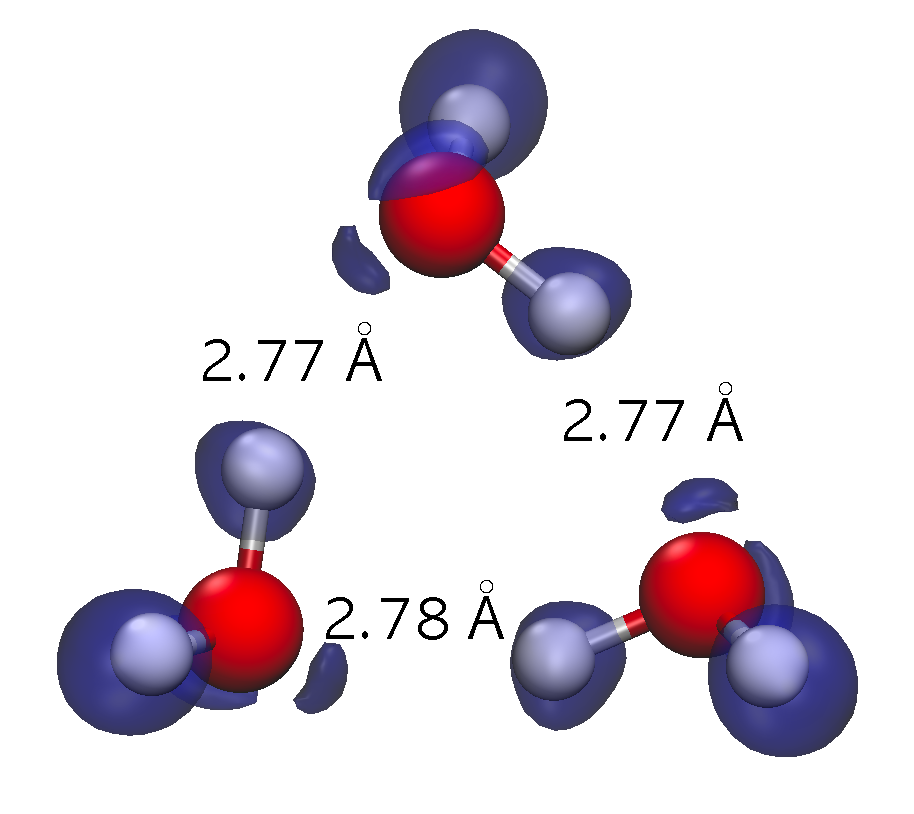
\includegraphics[width=\linewidth]{4/plots/elf/new/trimerELF}
    \caption{Water trimer.}
  \end{subfigure}
  \begin{subfigure}[b]{0.32\linewidth}
    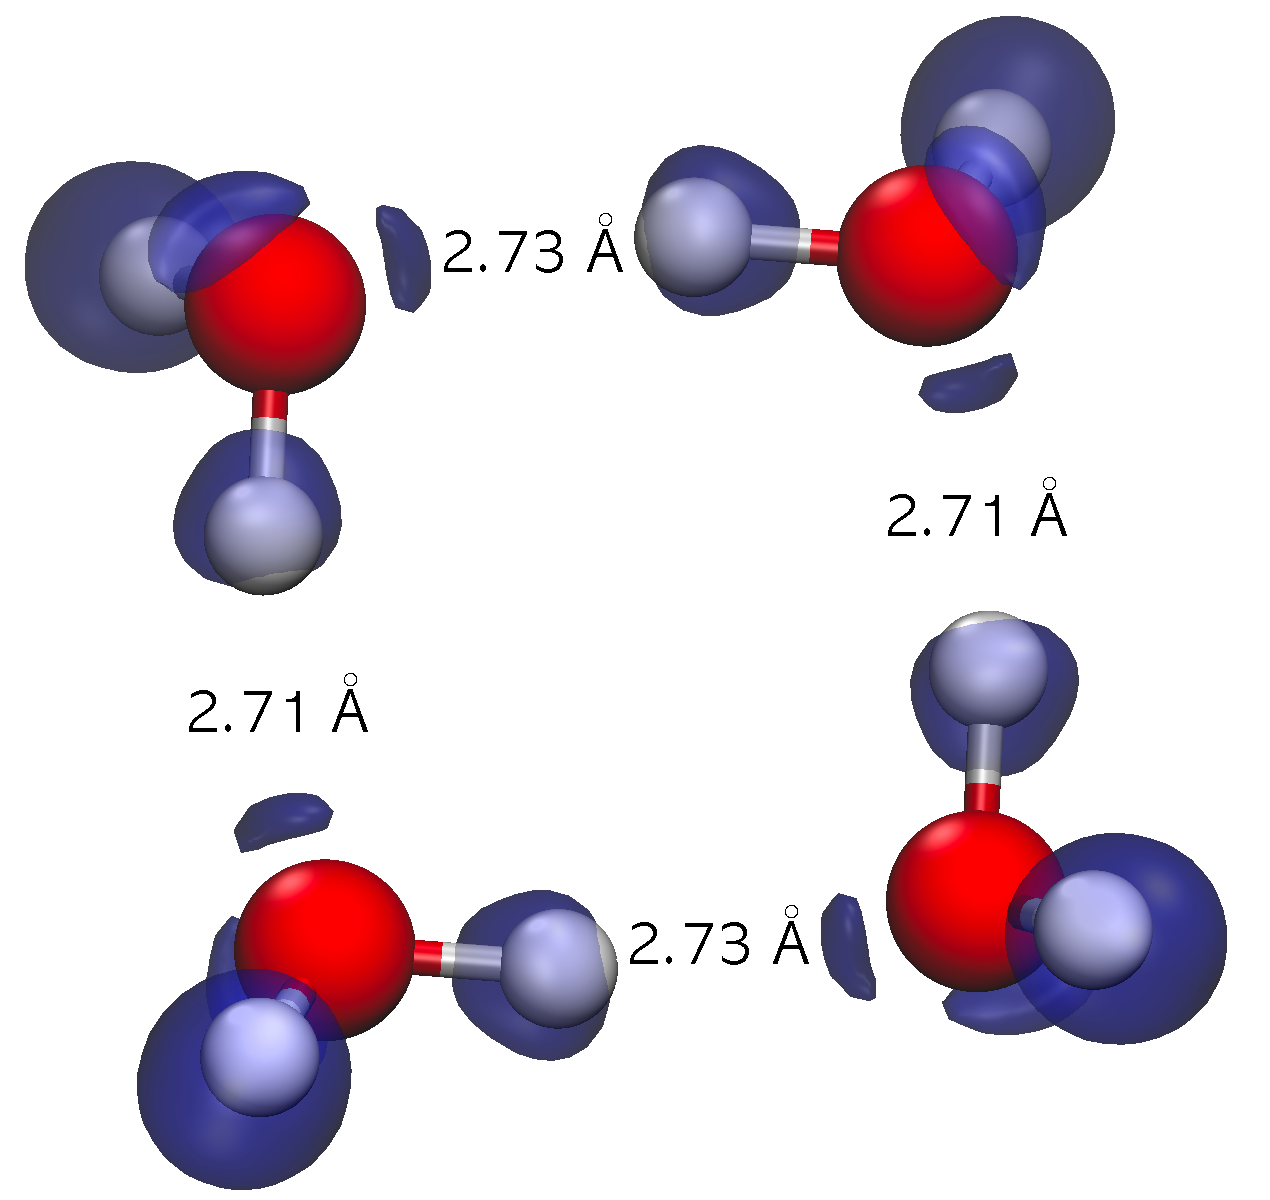
\includegraphics[width=\linewidth]{4/plots/elf/new/tetramer}
    \caption{Water tetramer.}
  \end{subfigure}
  \begin{subfigure}[b]{0.32\linewidth}
    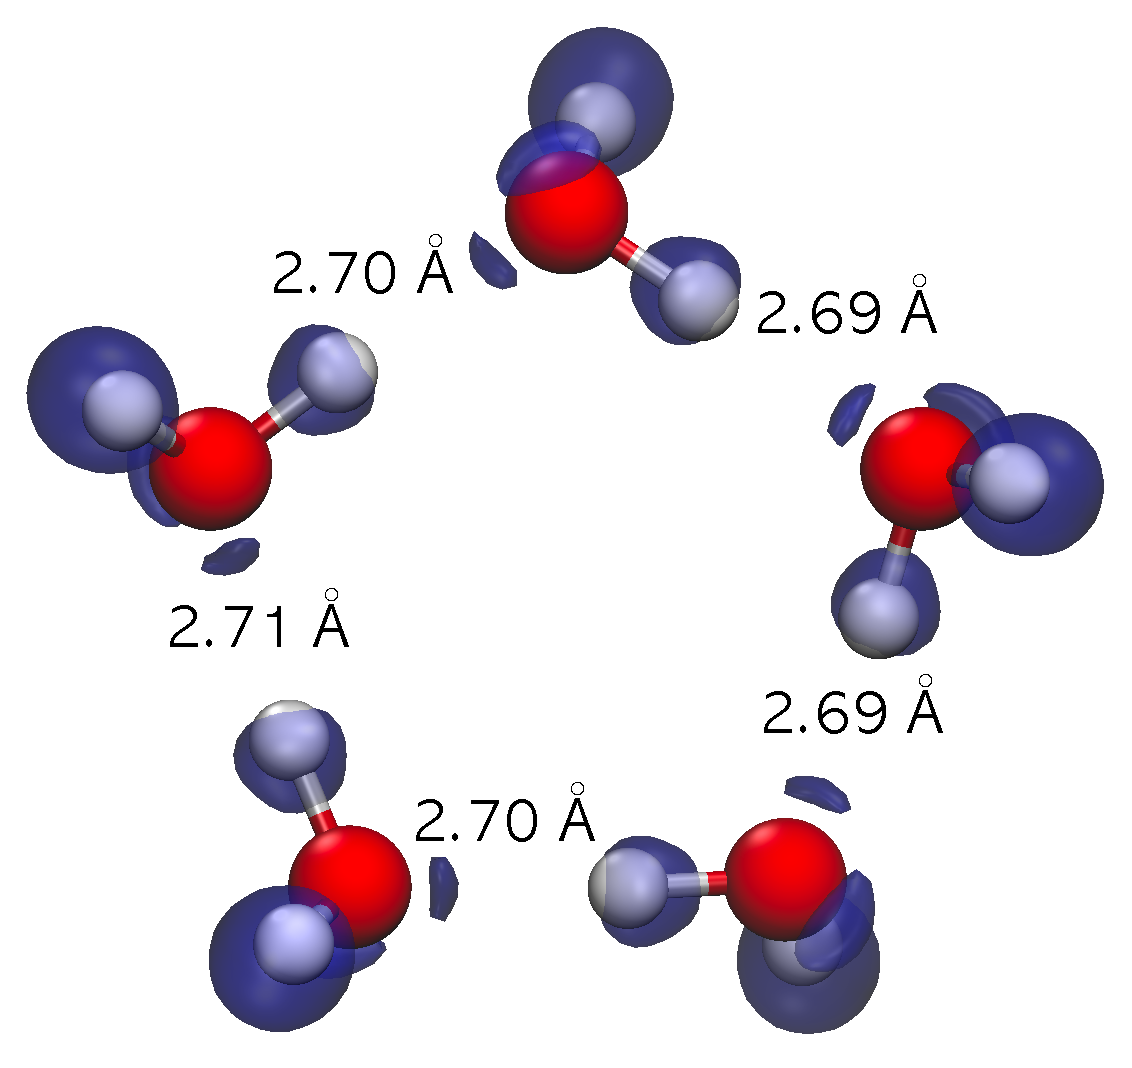
\includegraphics[width=\linewidth]{4/plots/elf/new/pentamer_cELF}
    \caption{Water cyclic pentamer.}
  \end{subfigure}
  \caption{Homodromic water clusters along with their corresponding hydrogen bond distances.}
  \label{homodromic}
\end{figure}

For homodromic clusters every molecule is acting as acceptor and as donor.  All
the density lost by the system as a donor is retrieved back as an acceptor.
Also the distances in the cluster (see Figure \ref{homodromic}) have a trend,
every time we add a new water molecule in the system the distance between
oxygen atoms is reduced, \textit{i. e.}, the HB is stronger, thus we can see
how the cooperativity is acting in the clusters.

\newpage

Pentamer p is nonetheless an exception. Indeed, the system not only has
bi-coordinated molecules, but also tri-coordinated ones. This happens in two
cases: $i$) double donor, $ii$) double acceptor.  These two sub-cases of
tricoordinated water molecules make the ELF look more similar in H atoms when
the water molecule is a double donor and similar for lone pairs when the water
molecule is a double acceptor.

\begin{figure}
  \centering
  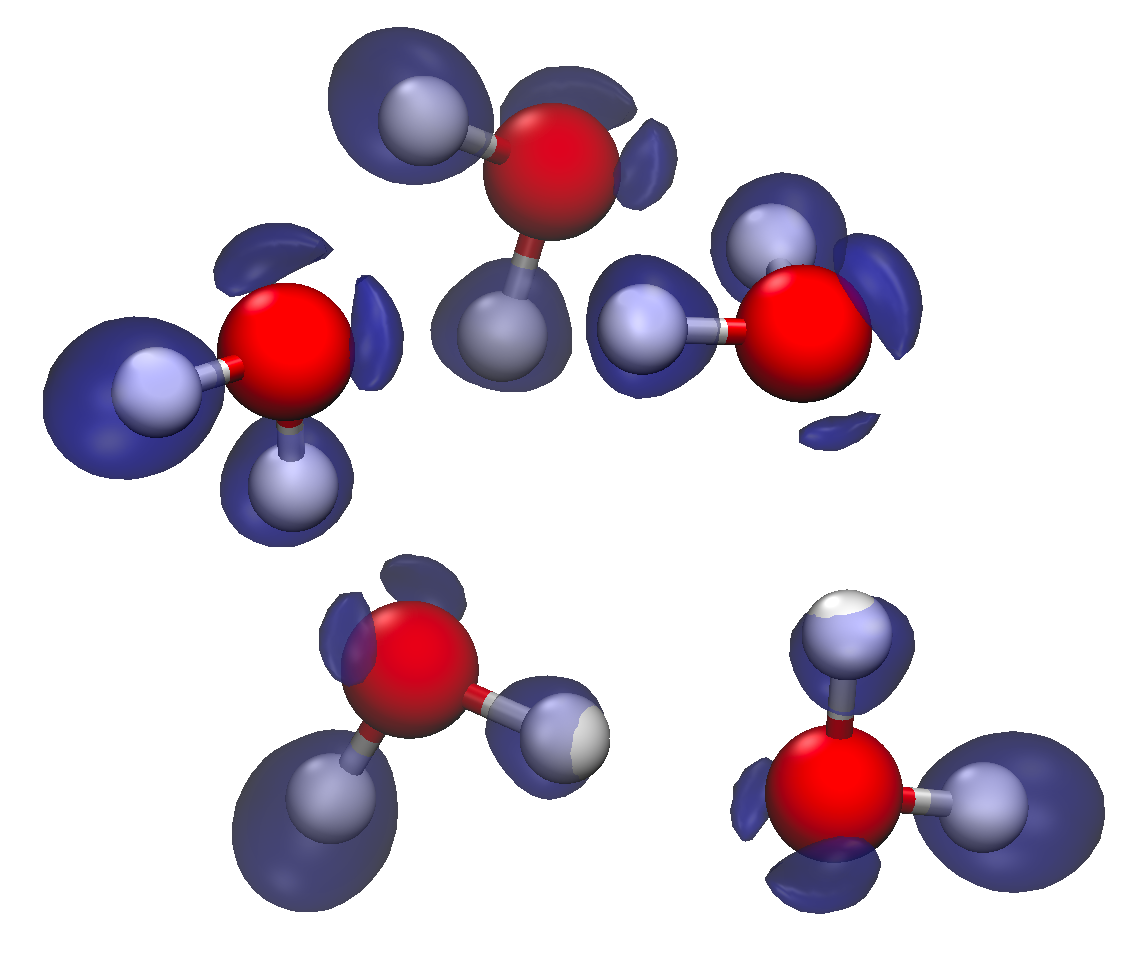
\includegraphics[width=0.4\textwidth]{4/plots/elf/new/pentamer_pELF}
  \caption{Polyhedric non-cyclic water pentamer (pentamer p).}
\label{pentamer_p}
\end{figure}

\newpage

\section{Non-Covalent Interactions}

The usual colour values for NCI are shown in the Figure
\ref{escala_deColorines} where the attractive strongest interactions are
shifted to blue and red, blue for attractive interactions and red for
repulsive.  For all our cases we have only strongly attractive interactions as
expected since the HB is a strongly attractive non-covalent interaction.

Looking at the NCI in water clusters, the dimer presents a prominent feature,
the only non-covalent interaction is the HB between the two water molecules,
the well-known HB in water clusters. The same pattern appears in the trimer and
tetramer with the addition of a small NCI region in the middle of the ring.

As we increase the number of water molecules in the cyclic clusters the NCI
volume is smaller for HB, as well as the NCI that lies in the middle of the
rings, this last type of NCI is enough small in the pentamer c (Figure
\ref{penta_c_nci}), that we changed the isosurface value to the plot, and
therefore, see the NCI region, while the other plots has a isosurface value
equals to 0.3, for the pentamer c is 0.5.

Pentamer p has the particularity that has different types of non-covalent
interactions, as we can see in Figure \ref{penta_p_nci} the system has four NCI
within the rings and one NCI inside the cage. Moreover, we can see how even if
the HBs are all blue coloured, they do not have the same volume, giving the
idea that are not all same.

\begin{figure}[h!]
  \centering
  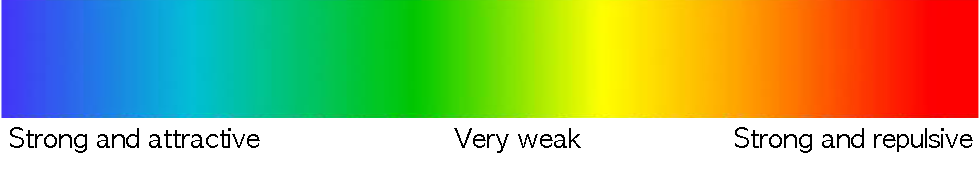
\includegraphics[width=0.8\textwidth]{4/plots/nci/escalita_NCI_colorines.png}
  \caption{Usual colour scale for NCI.}
\label{escala_deColorines}
\end{figure}

\begin{figure}[h!]
  \centering
  \begin{subfigure}[b]{0.32\linewidth}
    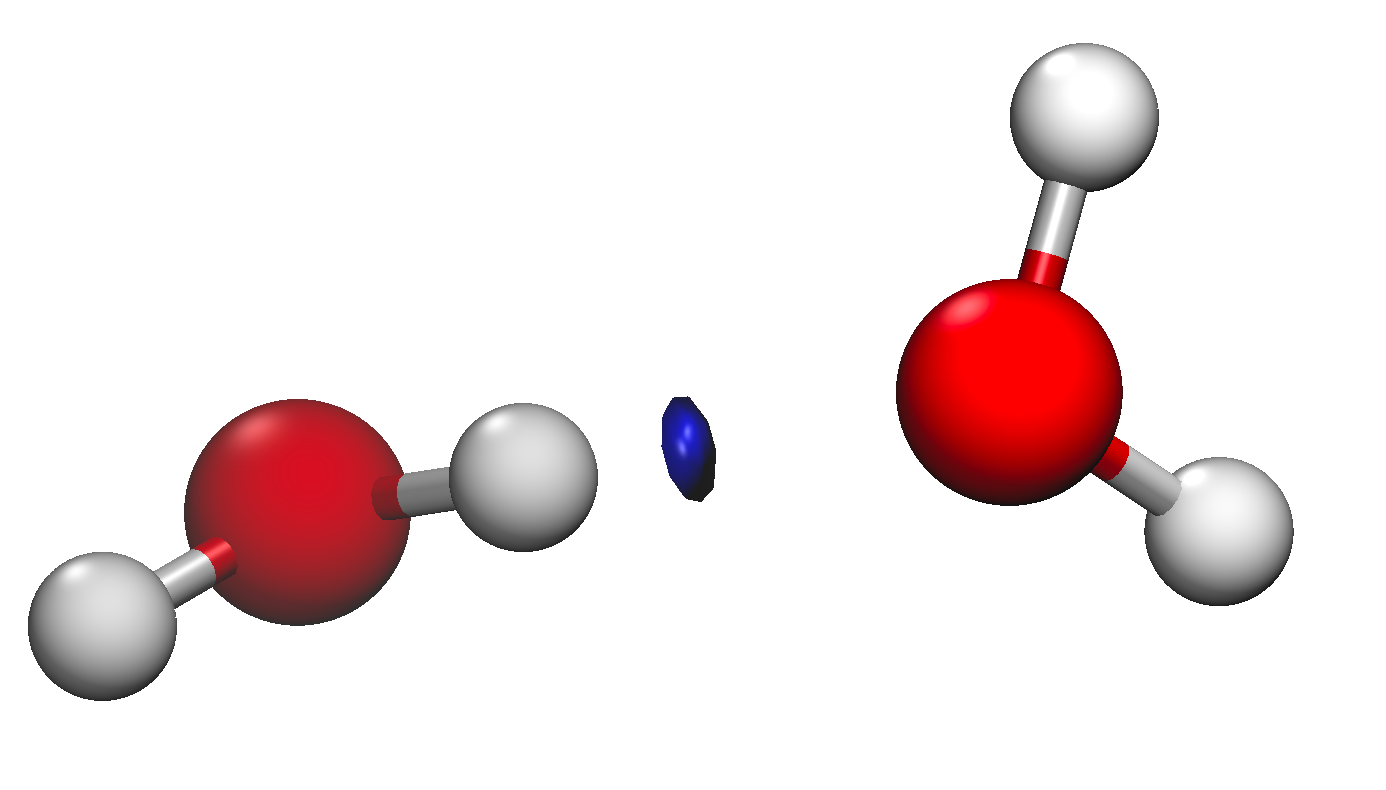
\includegraphics[width=\linewidth]{4/plots/nci/new/dimeroNCI}
    \caption{Water dimer.}
  \end{subfigure}
  \begin{subfigure}[b]{0.32\linewidth}
    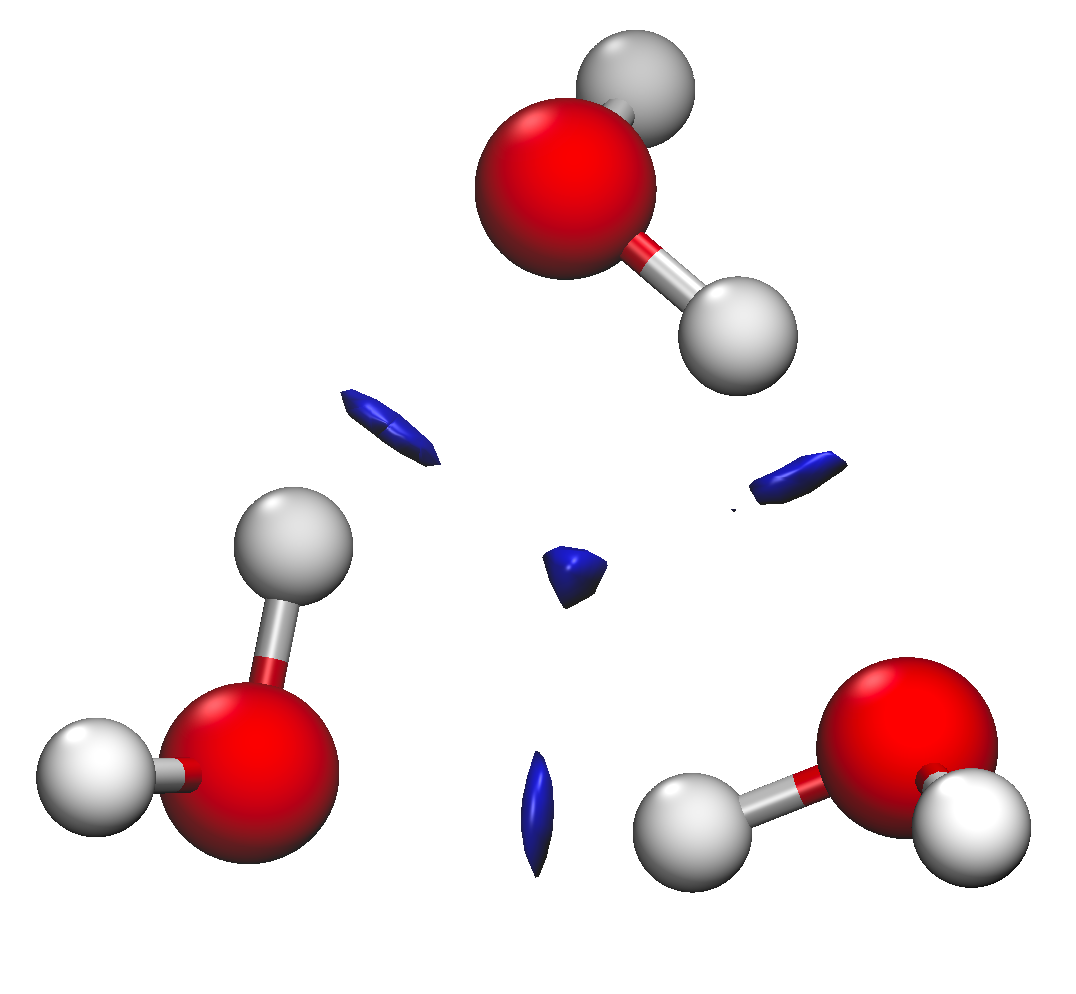
\includegraphics[width=\linewidth]{4/plots/nci/new/trimer}
    \caption{Water trimer.}
  \end{subfigure}
  \begin{subfigure}[b]{0.32\linewidth}
    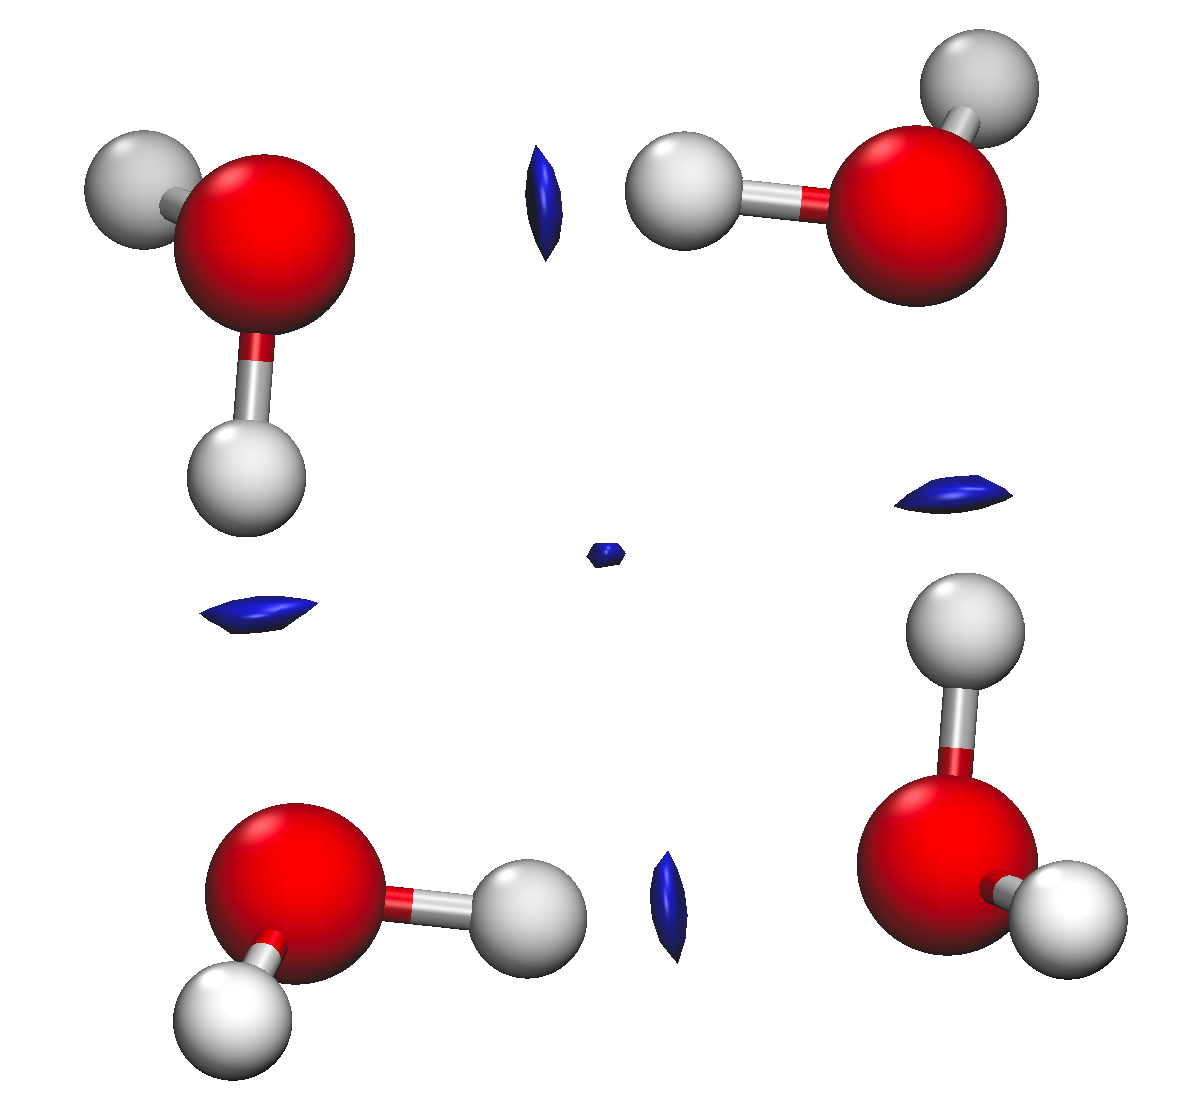
\includegraphics[width=\linewidth]{4/plots/nci/new/tetramerNCI}
    \caption{Water tetramer.}
  \end{subfigure}
  \begin{subfigure}[b]{0.4\linewidth}
    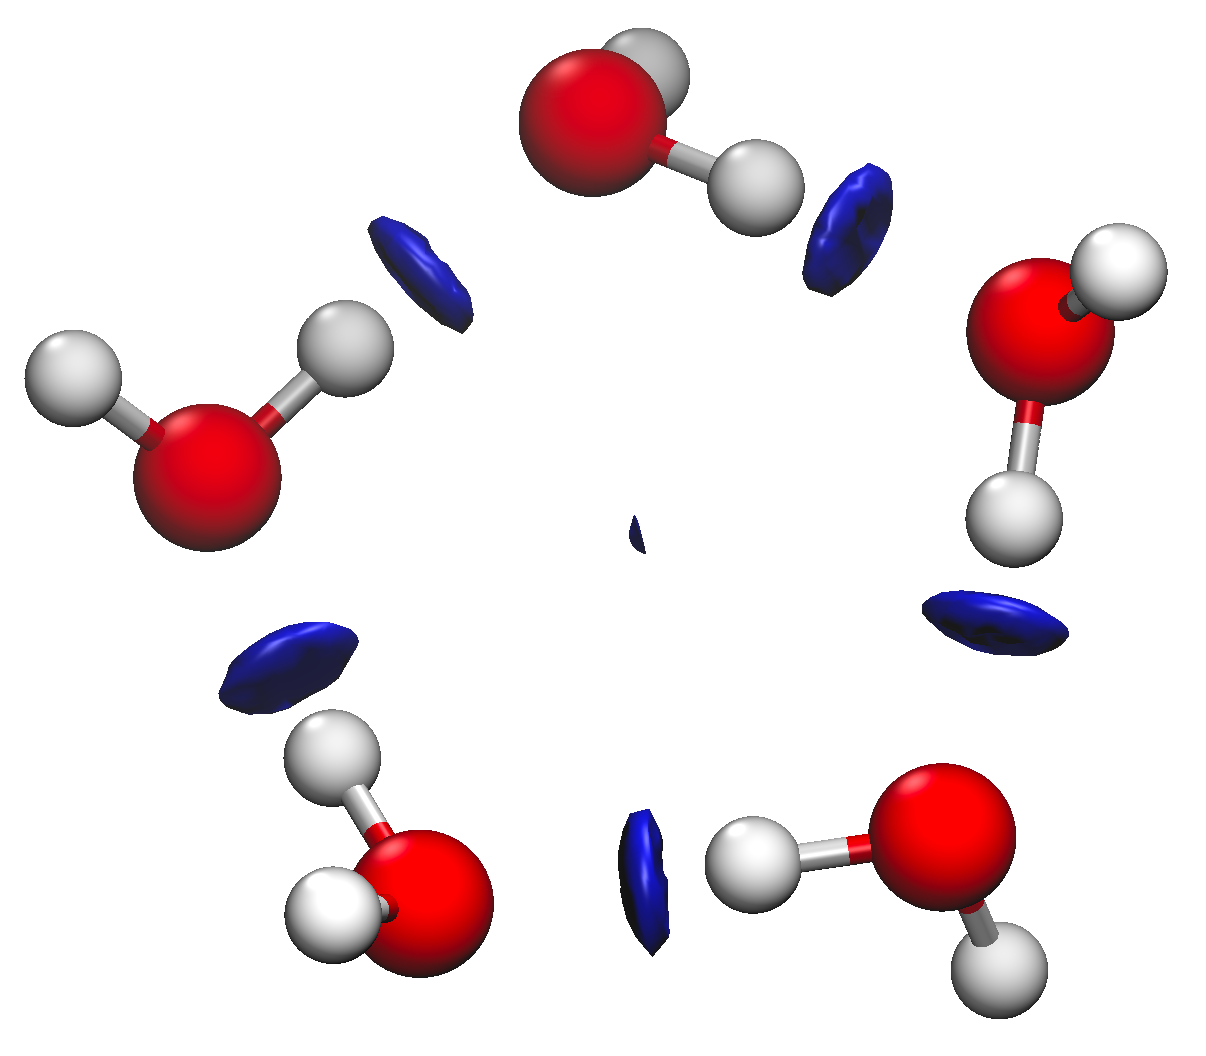
\includegraphics[width=\linewidth]{4/plots/nci/new/pentamer_cNCI}
    \caption{Water cyclic pentamer (pentamer c).}
    \label{penta_c_nci}
  \end{subfigure}
  \begin{subfigure}[b]{0.4\linewidth}
    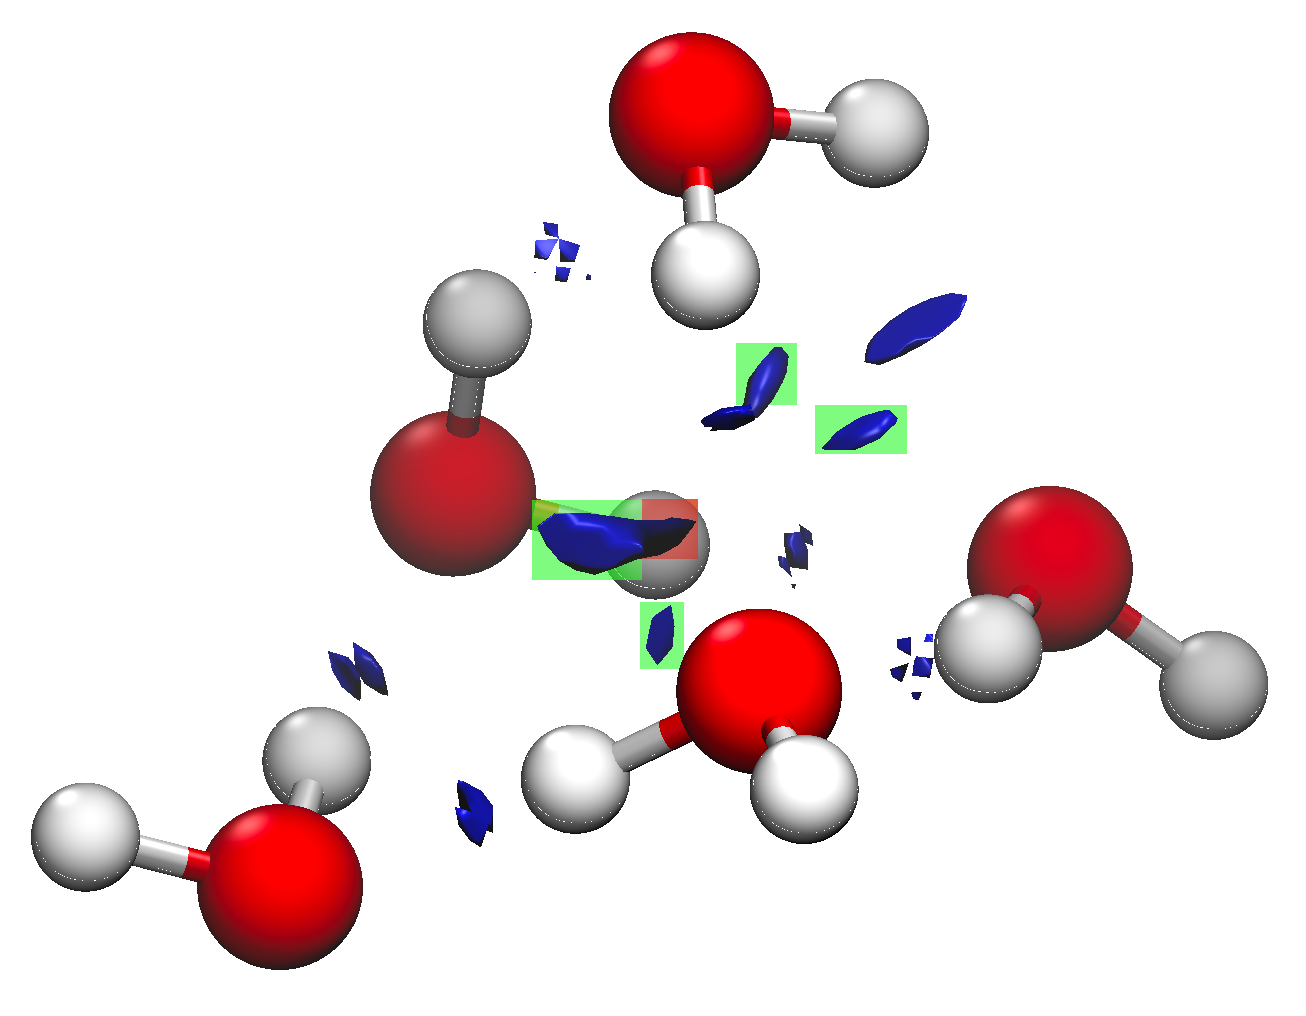
\includegraphics[width=\linewidth]{4/plots/nci/new/pentamer_pNCI}
    \caption{Water non-cyclic polyhedric pentamer (pentamer p).}
    \label{penta_p_nci}
  \end{subfigure}
  \caption{NCI method applied to Set 1 of water clusters. In Subfigures b, c and d the central isosurface is a RCP, while in
  Subfigure e the
  green highlight means a RCP, the red one is a CCP and the non highlighted interactions are HB.}
  \label{NCI}
\end{figure}


%\newpage
\clearpage

\section{{\sc{Promelf}}}

The next ELF analysis was done about its topology, particularly how the HB
interactions have their energy contributions as a function of their topology,
the topology analysis was given by {\sc{Promelf}}.

\begin{wrapfigure}{r}{0.5\textwidth}
    \centering
    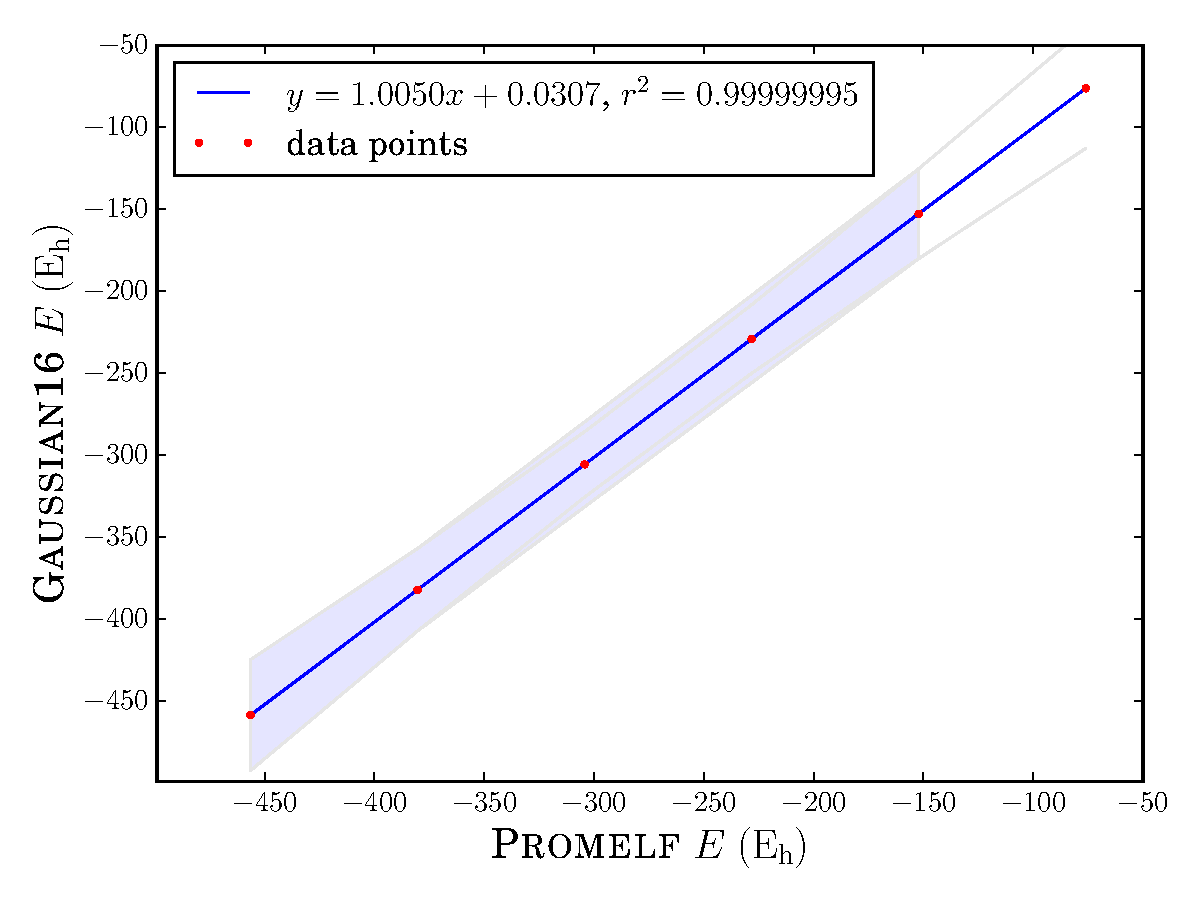
\includegraphics[width=0.5\textwidth]{4/plots/promelf/wfn_vs_promelf.pdf}
    \caption{Linear Regression between energy by {\sc{Gaussian16}} and {\sc{Promelf}} (atomic units).}
\label{rl_wfn}
\end{wrapfigure}

After fixing the computational problems discussed in Section \ref{SecTheory},
we carried out a security check of how different is the energy given by
{\sc{Promelf}} and the energy that {\sc{Gaussian16}}~\cite{g16} gives in the
\texttt{*wfn} files. To compare the values we did a linear regression (see
Figure \ref{rl_wfn}). The slope is  also near to one and the origin ordinate
is close to zero, the slope and the origin ordinate have an uncertainties near
to zero. Also the $r^2$ is really close to one. Hence, we can conclude that the
basin integrals are recovering the full system.

The most interesting thing that we can see with the data is how far or close
are the energy {\sc{Promelf}} values, and check their system-size dependency.
Most of the time we are 0.487 \% above the energy given by {\sc{Gaussian16}}
with a standard deviation of 0.014 \%.

To know more about these fluctuations and the differences between
{\sc{Promelf}} and {\sc{Gaussian16}} we have also plotted the values of the
energy divided per the number of water molecules that the system has.

As we can see in the Figure \ref{per_water_m}, {\sc{Gaussian16}} energy always
predicts a negative $\Delta E$, while {\sc{Promelf}} predicts a positive one.
Hence, the $\Delta E$ by {\sc{Promelf}} (and $\Delta G$ with {\sc{Gaussian16}})
cannot be used to predict if a system is energetically favorable for water
clusters since the anharmonic contributions cannot be neglected and these
contributions are not taken into account in the two
software~\cite{MuozCaro1997}.

\begin{figure}[h]
  \begin{minipage}[t]{0.47\textwidth}
    \centering
    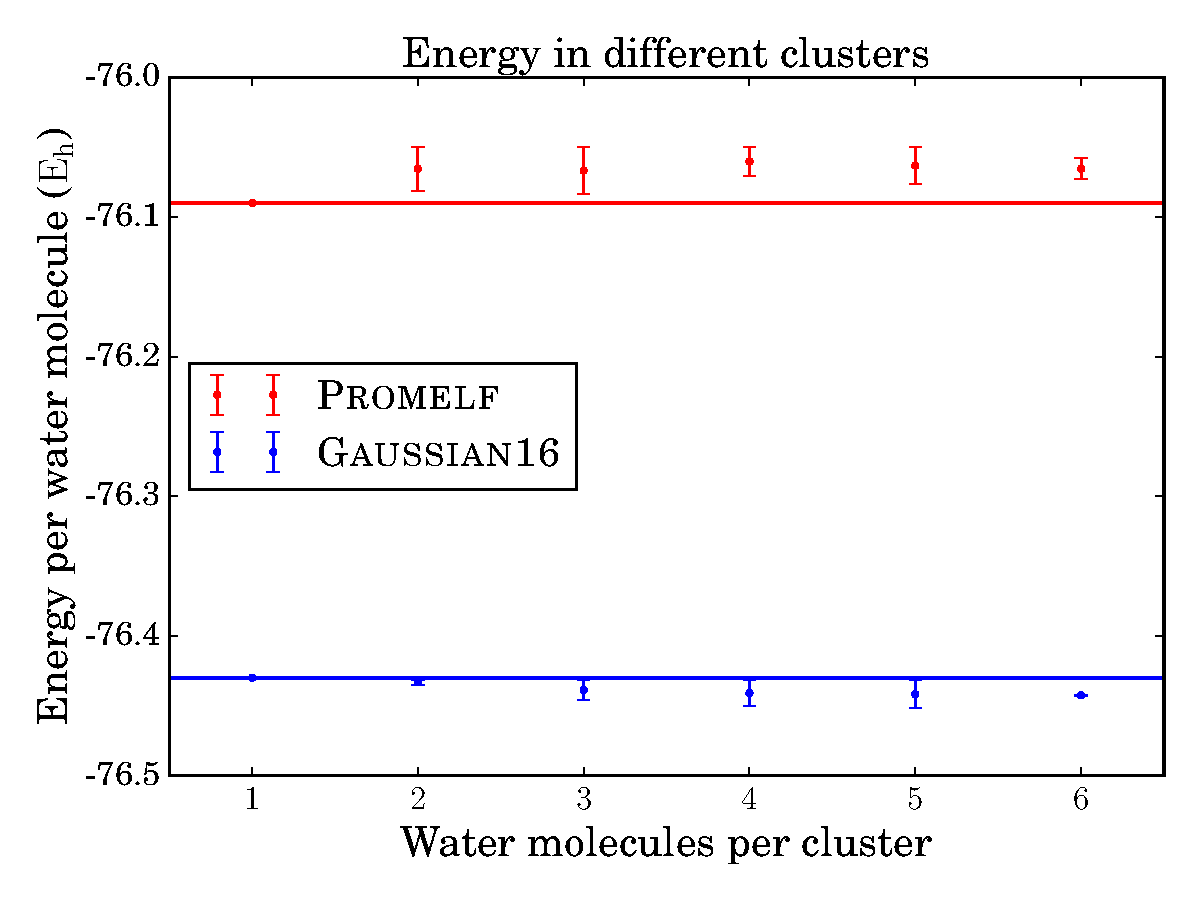
\includegraphics[width=\textwidth]{4/plots/promelf/devided.pdf}
    \caption{Energy of clusters divided by the number of water molecules [Sets 1, 2 and 3]. The two horizontal lines
    are the energy of one water molecule.}
    \label{per_water_m}
\end{minipage}
\hfill
\begin{minipage}[t]{0.47\textwidth}
    \centering
    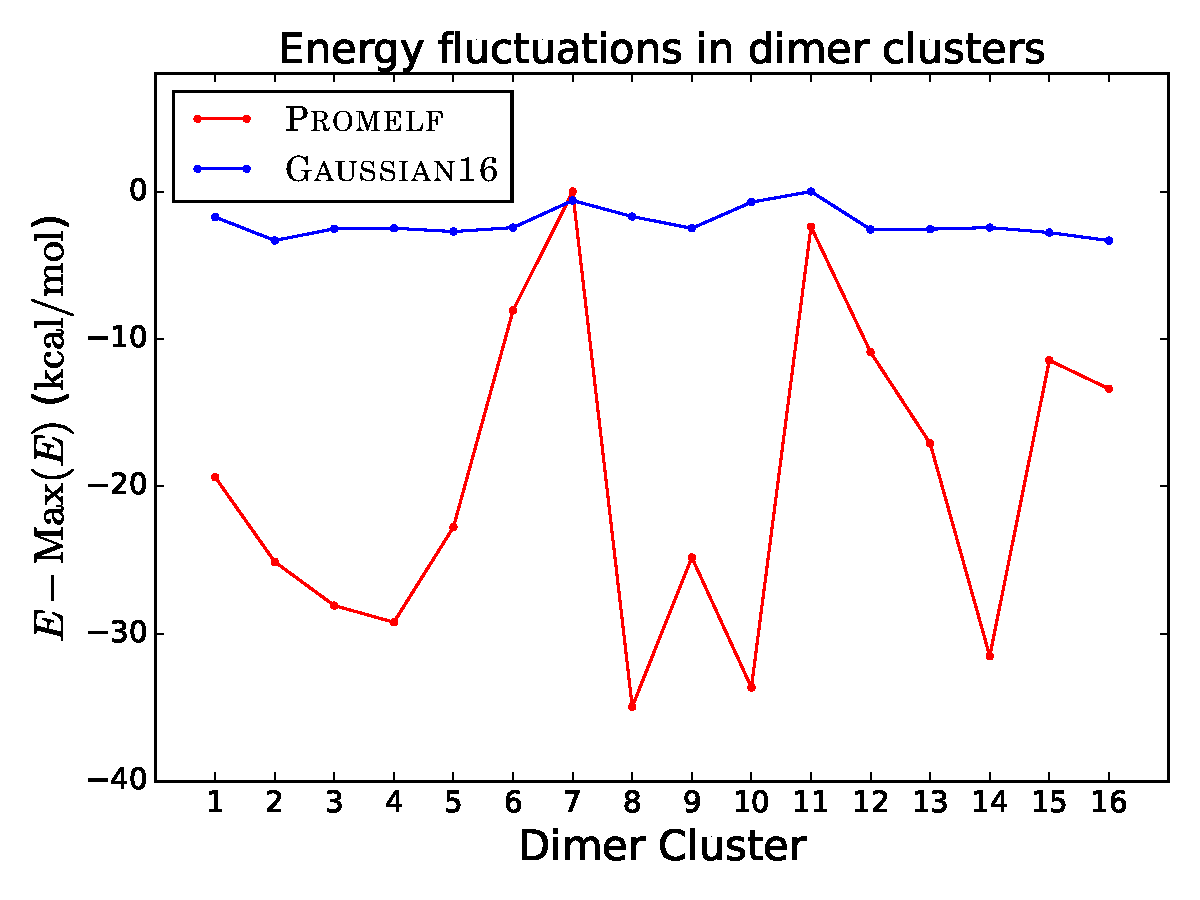
\includegraphics[width=\textwidth]{4/plots/promelf/dimer_energywfn.pdf}
    \caption{{\sc{Promelf}} and {\sc{Gaussian16}} energy fluctuation of water dimers.}
    \label{fluctuations}
\end{minipage}
\end{figure}

\newpage

Figure \ref{fluctuations} compares the energy fluctuation in dimers (Set 2)
provided by {\sc{Promelf}} and {\sc{Gaussian16}}. This set allows a systematic
assessment of the energy for a same system with different aggregate
configurations. As evidence by the picture, the {\sc{Promelf}} line presents
strong oscillations of several \SI{}{\kilo\calorie\per\mole}, in clear contrast
with the results provided by {\sc{Gaussian16}}. Moreover, the minimum and the
maximum do not correspond to the same systems.

One property that has the same behavior as the energy computed by
{\sc{Gaussian16}} is the exchange-correlation contribution in the HB
interactions as we can see in the Figures \ref{dimer_b_w_g} and
\ref{dimer_b_w_xc}, where particularly the minimum and maximum are the same
systems in the two cases.

However, their relation is not 100 \% correlated as we can see through a linear
regression (Figure \ref{dimer_b_w_rl}), having $r^2 = 0.84$ for the equation $y
= 1.3335x + 203.8$.

\begin{figure}[h]
    \begin{minipage}[t]{0.47\textwidth}
      \centering
      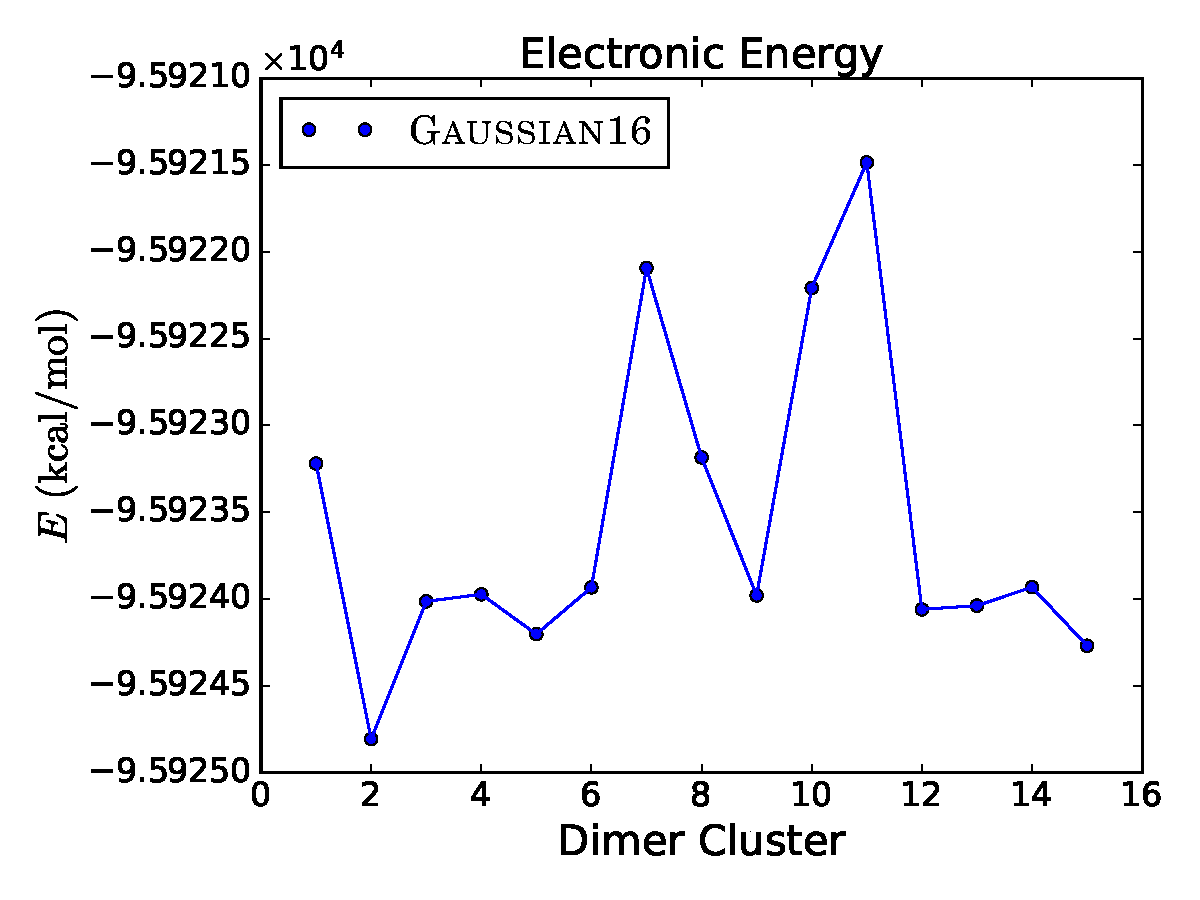
\includegraphics[width=\textwidth]{4/plots/promelf/wfn_dimer_trend.pdf}
      \caption{Electronic Energy for Dimer Clusters computed by {\sc{Gaussian16}}.}
      \label{dimer_b_w_g}
    \end{minipage}%
    \hfill
    \begin{minipage}[t]{0.47\textwidth}
      \centering
      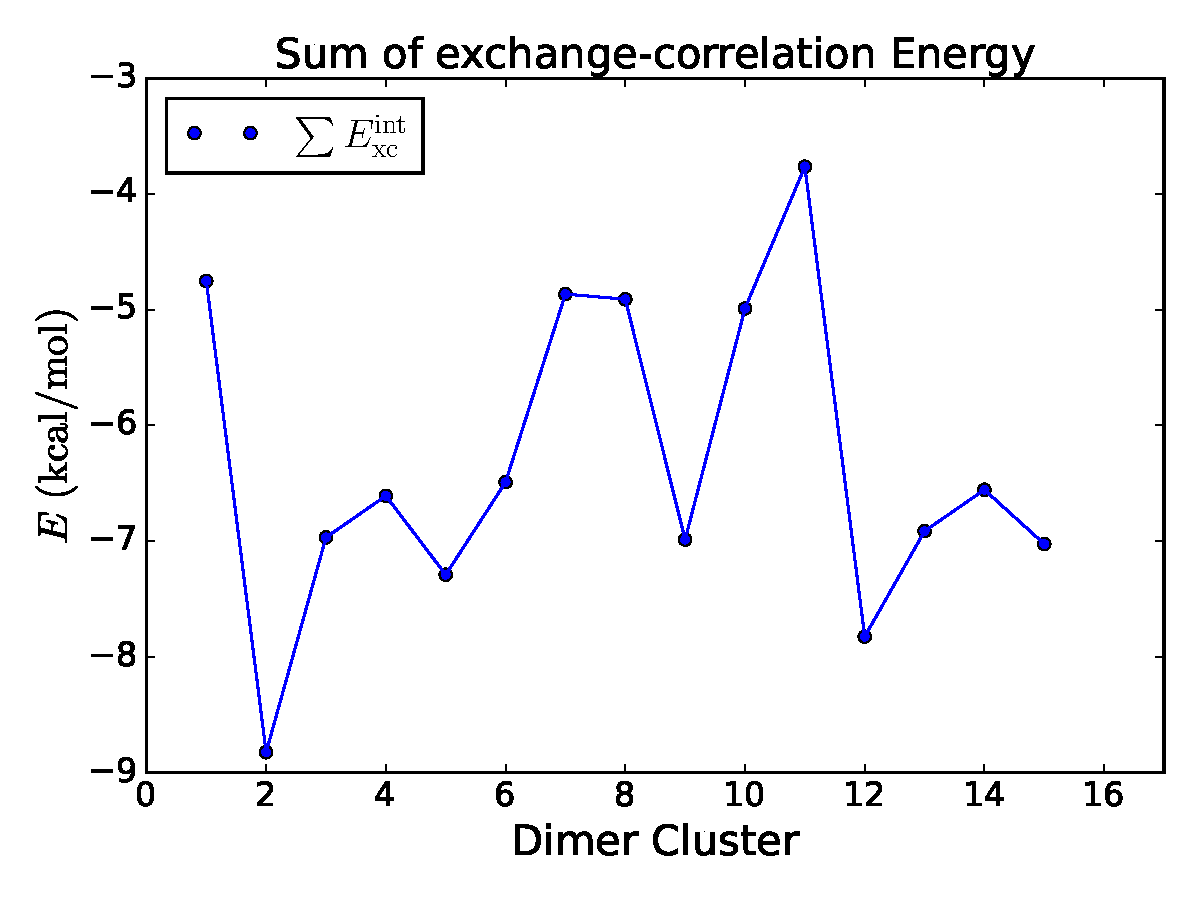
\includegraphics[width=\textwidth]{4/plots/promelf/xc_int.pdf}
      \caption{Exchange-correlation interaction energy for Dimer Clusters.}
      \label{dimer_b_w_xc}
    \end{minipage}%
\end{figure}
\begin{figure}[h]
    \begin{minipage}[t]{0.50\textwidth}
      \centering
      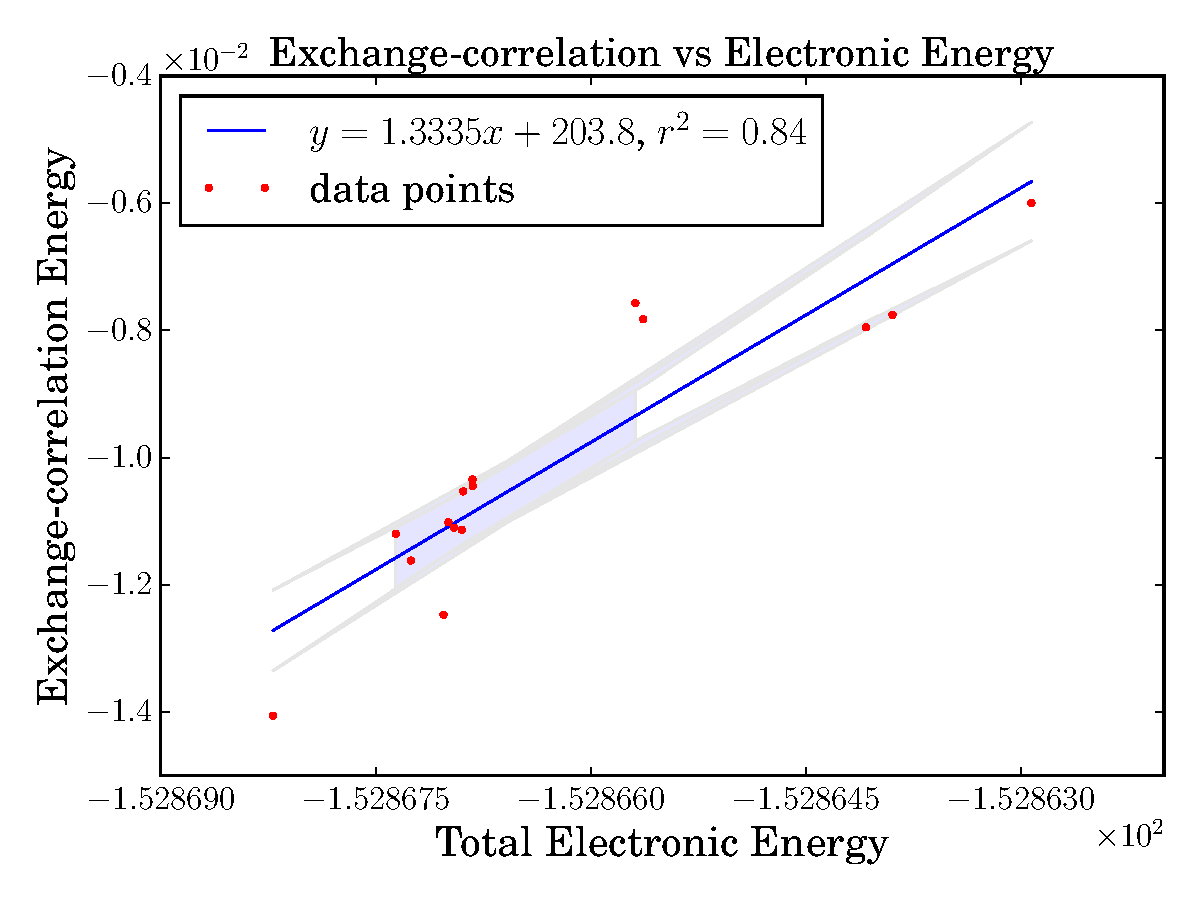
\includegraphics[width=\textwidth]{4/plots/promelf/wfn_xc}
      \caption{Linear regression between exchange-correlation contribution in interaction
      and electronic energy for whole system.}
      \label{dimer_b_w_rl}
    \end{minipage}%
    \hfill
    \begin{minipage}[t]{0.4\textwidth}
      \centering
      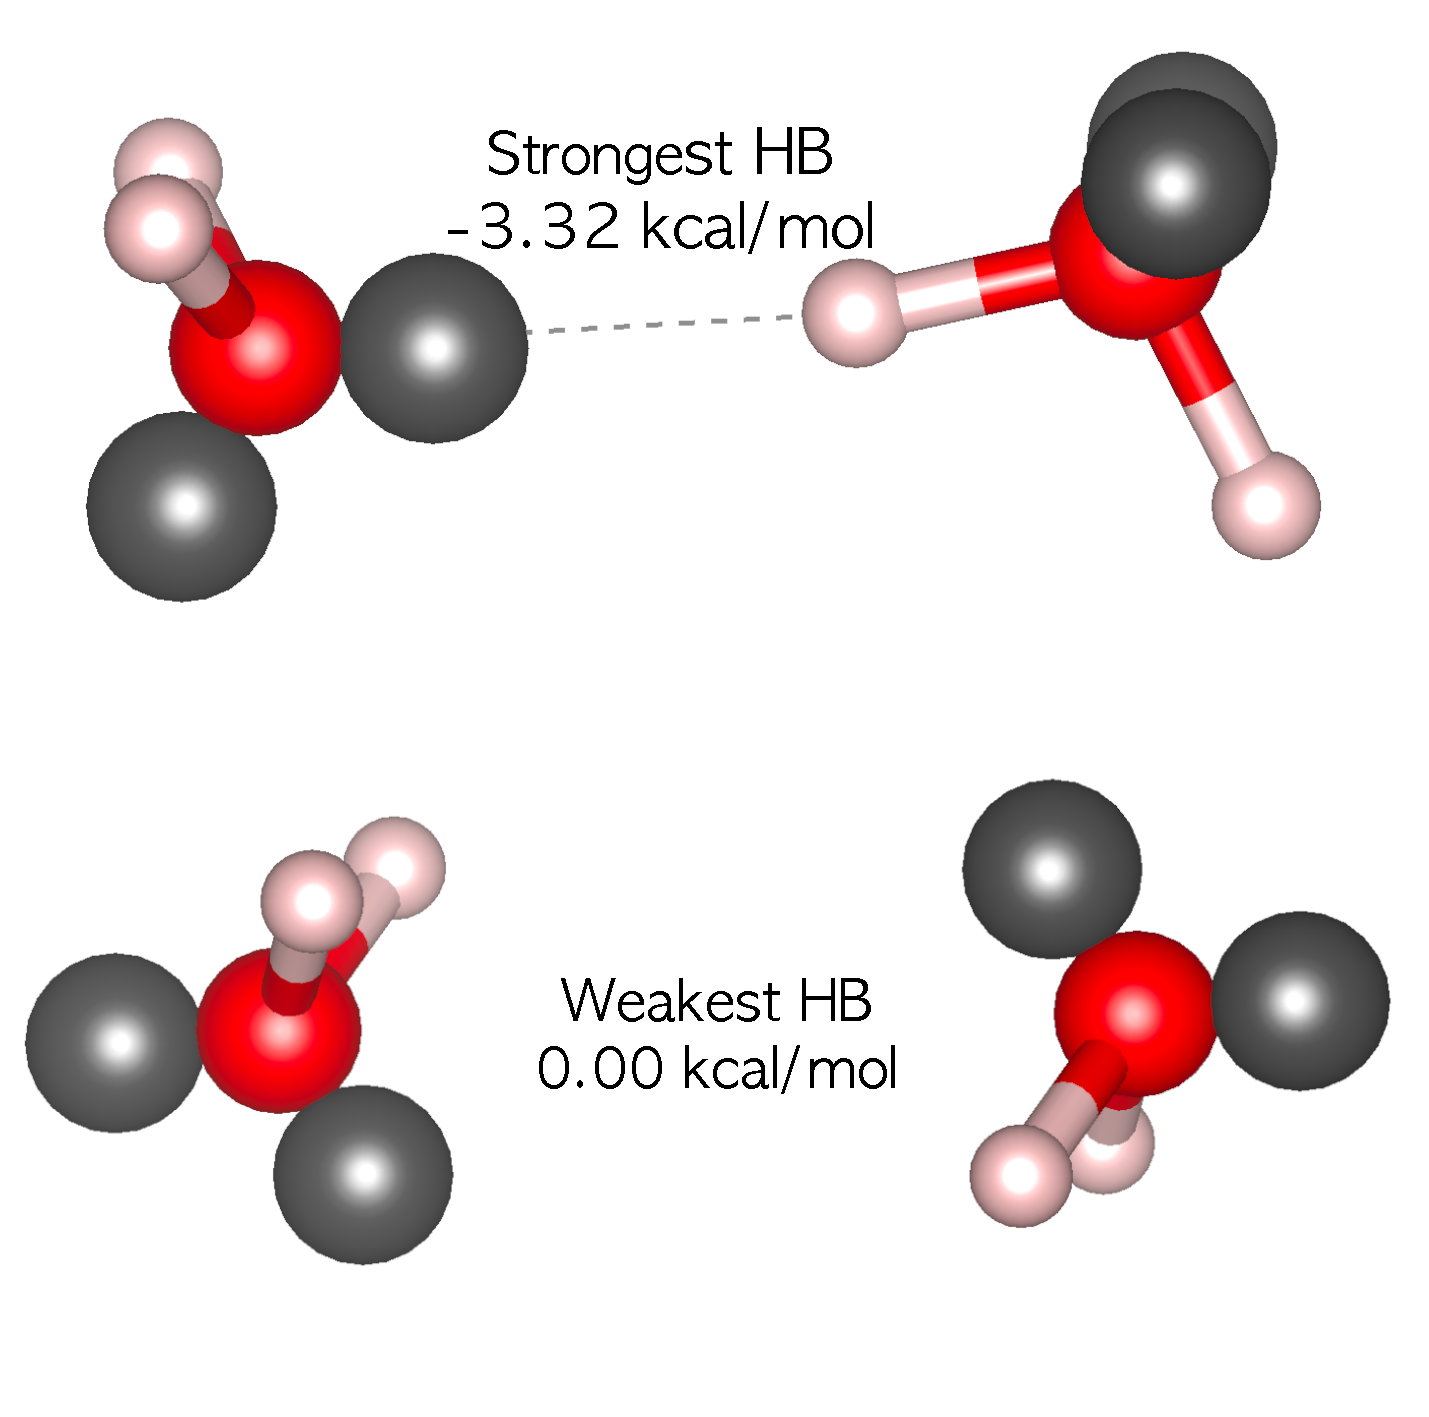
\includegraphics[width=\textwidth]{4/plots/dibujitos/dimers_b_w}
      \caption{Strongest and weakest HB in water dimer clusters and their relative electronic energy.}
      \label{dimer_b_w_t}
    \end{minipage}%
\end{figure}

As we said, the maximum and the minimum for the two cases are the same system.
These two extreme cases correspond to the weakest and the strongest HB for any
water dimer cluster computed. Therefore, the minimization/maximization of the
energy are completely related with the exchange-correlation energy of HB.  The
two cases are shown in Figure \ref{dimer_b_w_t}, the difference of the two
systems is \SI{3.32}{\kilo\calorie\per\mole} of the total electronic energy,
and 5.05 \si{\kilo\calorie\per\mole} for the exchange-correlation contribution.

\newpage

To compute the exchange-correlation contribution, the various interactions
between H and electron pairs were taken into account and not just the values
coming from the classical HB (even if that was the largest contribution).

Looking for the population we did two analyses, one with the delocalization
index (DI) and another one with the charge. The DI gives a quantitative idea of
the number of electrons delocalized or shared between atoms and the charge is a
measurement of how much the electrons are localized in the basins.

\newpage

\begin{figure}[th]
    \begin{minipage}[t]{0.47\textwidth}
      \centering
      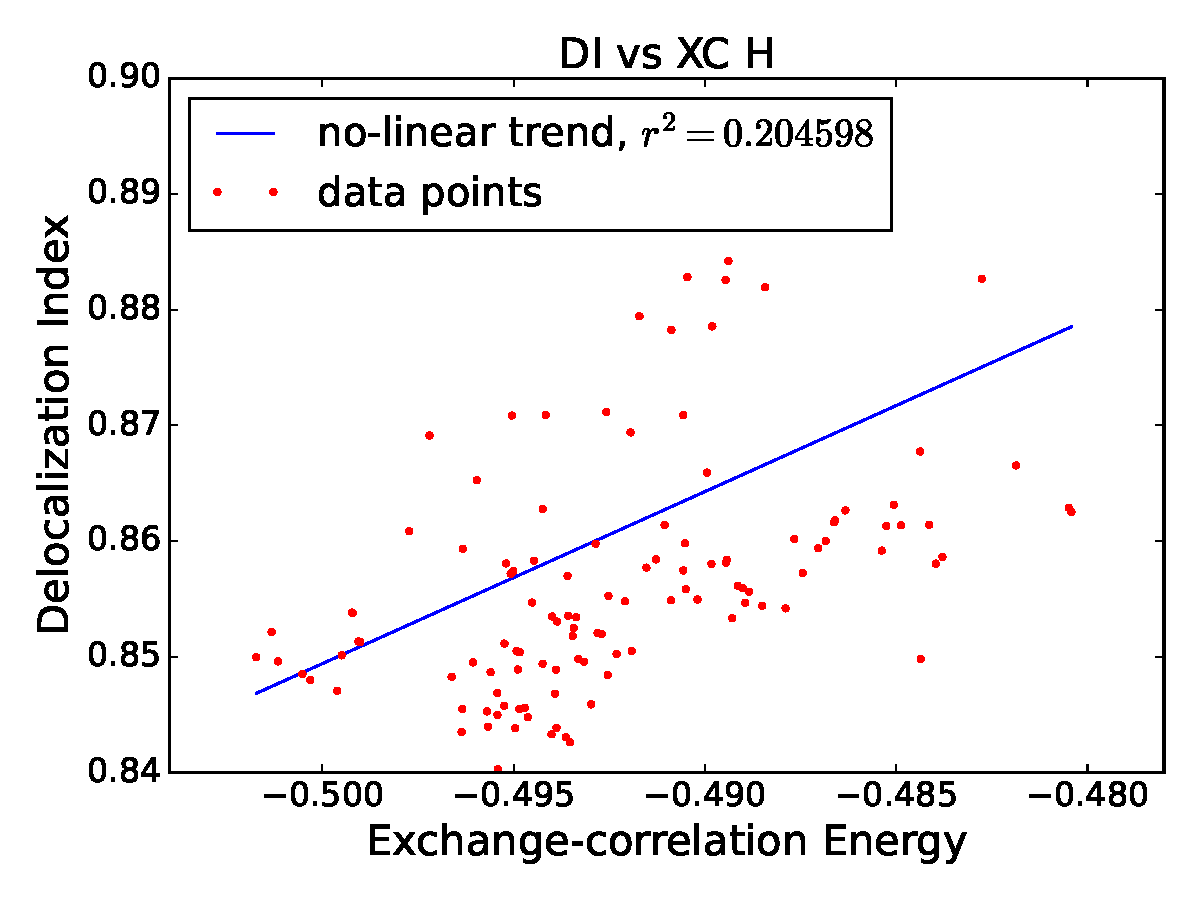
\includegraphics[width=\textwidth]{4/plots/promelf/xc_di_h.pdf}
      \caption{Linear regression between exchange-correlation energy
      and DI in H basin.}
      \label{di_xc_h}
    \end{minipage}%
    \hfill
    \begin{minipage}[t]{0.47\textwidth}
      \centering
      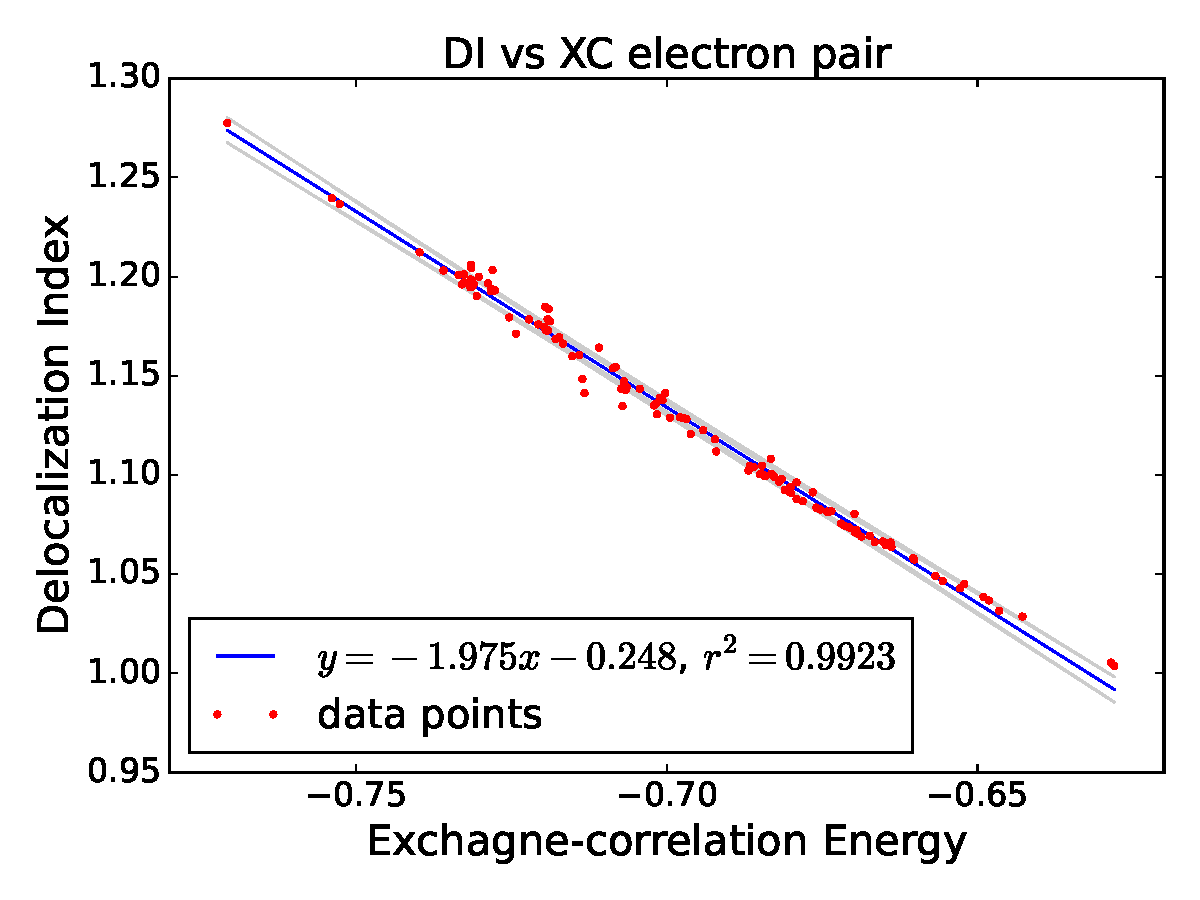
\includegraphics[width=\textwidth]{4/plots/promelf/xc_di_e.pdf}
      \caption{Linear regression between exchange-correlation energy
      and DI in lone pair electron basin.}
      \label{di_xc_e}
    \end{minipage}%
\end{figure}

With the delocalization index, we looked how the exchange-correlation energy is
correlated with the the delocalized electrons.  Having two different behavior
cases. The first one, where the DI and the exchange-correlation energy are
really well correlated with the ELF maximum basin associated to the lone
electron pair in HB's, with a $r^2 = 0.9923$. However, there is not any
correlation for the same phenomenon if we use the ELF maximum basin associated
with the H atom ($r^2 = 0.204598$). These two correlations are shown in Figures
\ref{di_xc_h} and \ref{di_xc_e}.

\begin{figure}[b!]
    \begin{minipage}[t]{0.48\textwidth}
      \centering
      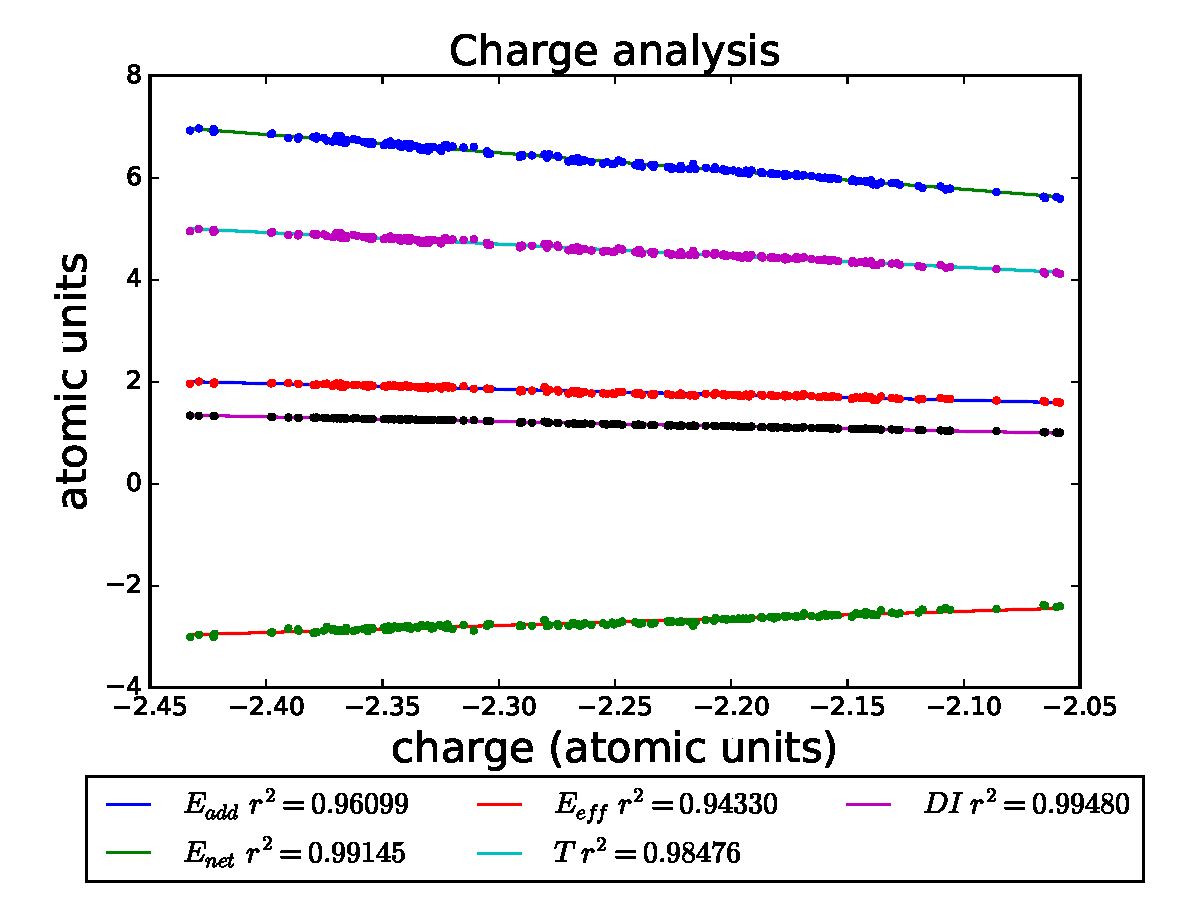
\includegraphics[width=\textwidth]{4/plots/promelf/charge/chargee.pdf}
      \caption{Linear regression about charge for lone pair electron basin.}
      \label{rl_chargee}
    \end{minipage}%
    \hfill
    \begin{minipage}[t]{0.48\textwidth}
      \centering
      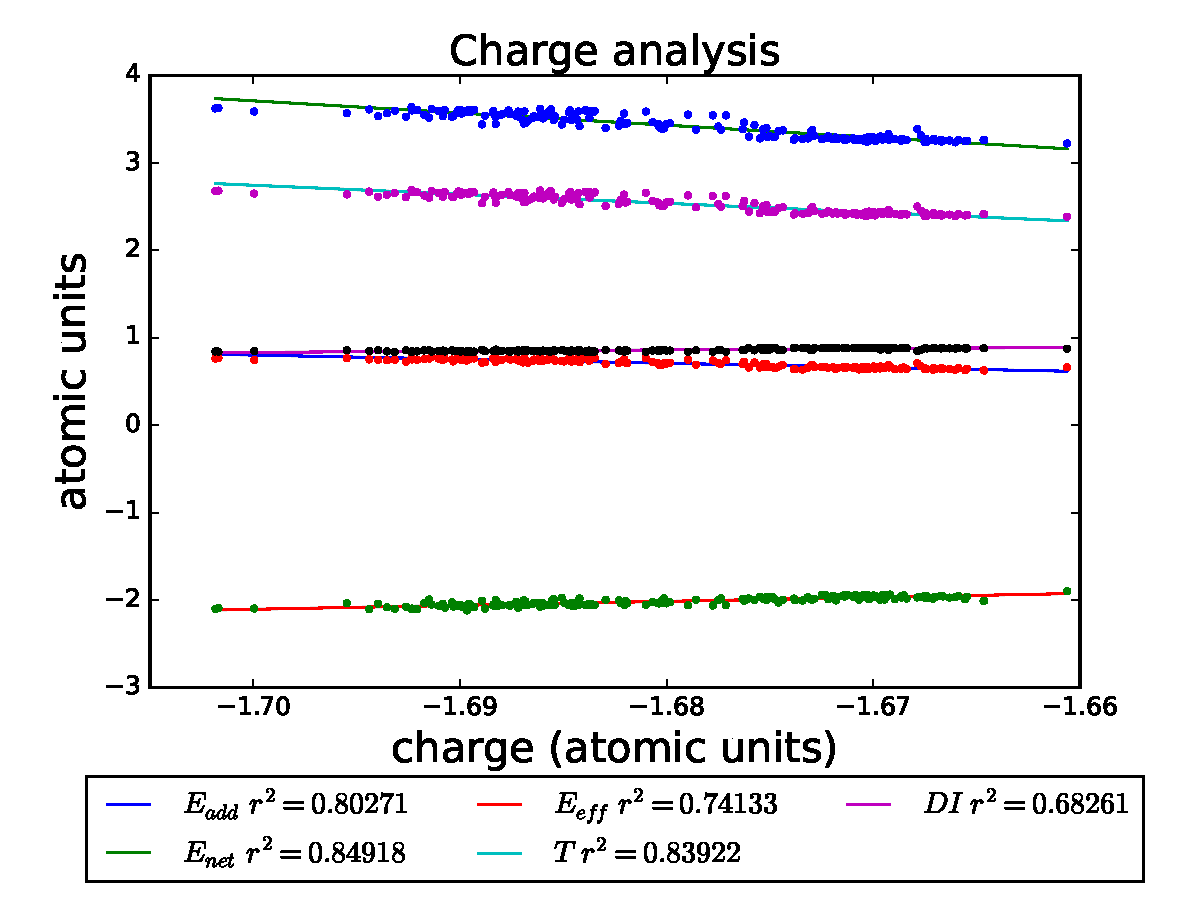
\includegraphics[width=\textwidth]{4/plots/promelf/charge/chargeH.pdf}
      \caption{Linear regression about charge for H basin.}
      \label{rl_chargeH}
    \end{minipage}%
\end{figure}

%\newpage
\pagebreak

We also checked how the properties of the basins correlate within the same
basin. For that in Figures \ref{rl_chargee} and \ref{rl_chargeH} we plotted
linear regressions of the charge versus:
$i$) kinetic energy,% ($T$),
$ii$) net energy $E_{\mathrm{net}}$, as exposed by IQA partition in Section \ref{IQAtheory} (Equation \ref{eAtomo}),
$iii$) effective energy $E_{\mathrm{eff}}^A=E_{\mathrm{net}}^A + \sum_{A\neq B}E_{\mathrm{int}}^{AB}$,
$iv$) additive energy $E_{\mathrm{eff}}^A=E_{\mathrm{net}}^A + \frac12 \sum_{A\neq B}E_{\mathrm{int}}^{AB}$, %($\sum E_{add} = E_{ele}$),
and $v$) DI.
The above for both the H basin and the electron pair basin.  We can see once
again, how the basins associated to lone pairs correlates with the charge and
the other properties, while for H basins there is from little to no correlation
(\textit{e. g.} DI).

\begin{wrapfigure}{l}{0.47\textwidth}
    \centering
    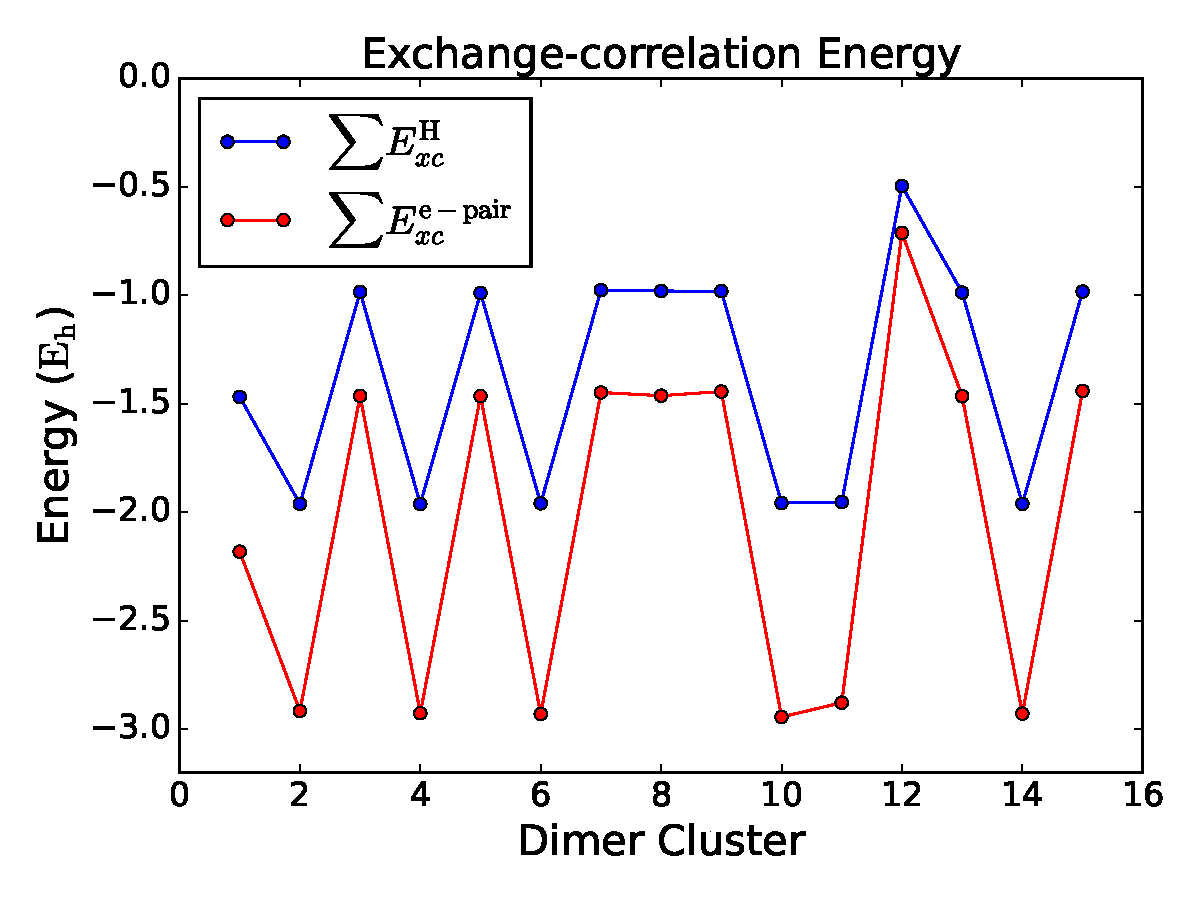
\includegraphics[width=0.48\textwidth]{4/plots/promelf/xc1_xc2.pdf}
    \caption{Trend of the sum of Exchange-Correlation Energy contribution
    for dimer systems.}
\label{xcHxcE}
\end{wrapfigure}


Looking at the dimer systems (Set 2) we did not find any correlation among the
energy contributions of HB. However, we found the same trend over the addition
of all HB contributions.  For example, the exchange-correlation contributions
sum for lone pairs has the same trend as the same contributions sum for H
basin. The above for all dimers, as we can see in Figure \ref{xcHxcE}.  Even if
the total energy does not follow any trend in the dimers, the
exchange-correlation contribution follows a trend over the electron pair and H
basins.

Based on these results, we decided to check for all sets the sum over the
kinetic, potential and exchange-correlation contributions to the total energy.
A linear regression between the sum of each of these three energy contributions
and the two ELF maxima (See Figure \ref{rlineales}).

\begin{figure}[hb]
     \centering
     \begin{subfigure}[b]{0.32\textwidth}
         \centering
         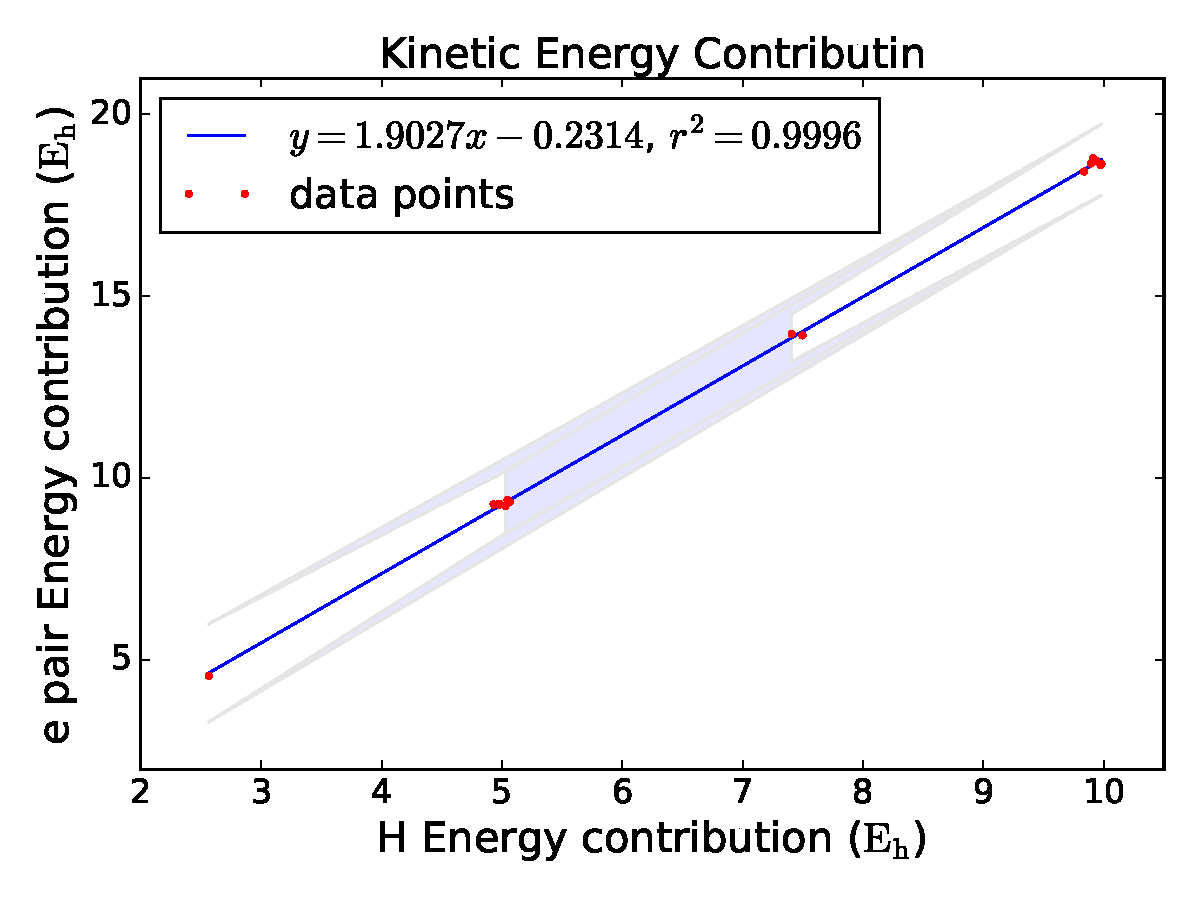
\includegraphics[width=\textwidth]{4/plots/promelf/rl_t1_t2}
     \end{subfigure}
     \hfill
     \begin{subfigure}[b]{0.32\textwidth}
         \centering
         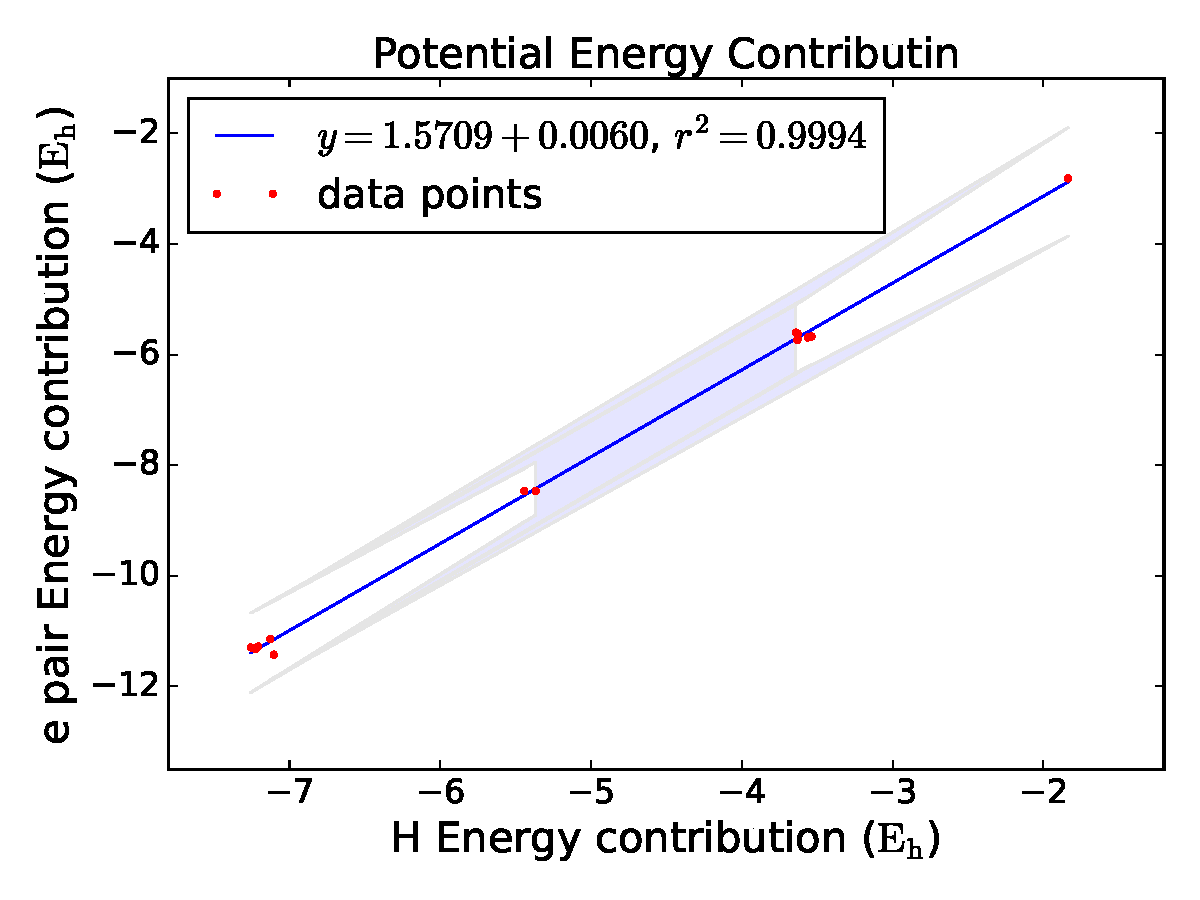
\includegraphics[width=\textwidth]{4/plots/promelf/rl_v1_v2}
     \end{subfigure}
     \hfill
     \begin{subfigure}[b]{0.32\textwidth}
         \centering
         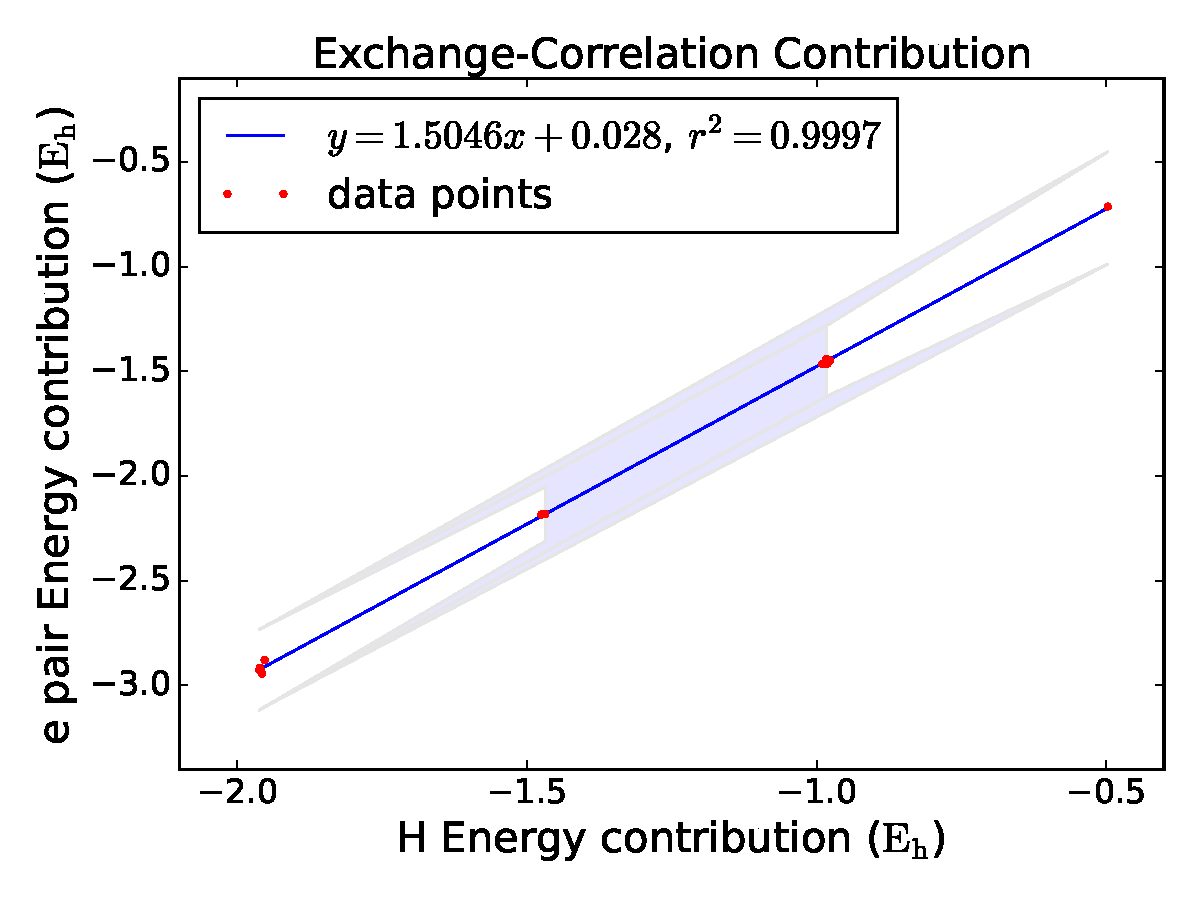
\includegraphics[width=\textwidth]{4/plots/promelf/rl_xc1_xc2}
     \end{subfigure}
        \caption{Linear Regressions between electron pair and H basins.}
        \label{rlineales}
\end{figure}

%\newpage
\pagebreak

\begin{wrapfigure}{r}{0.5\textwidth}
    \centering
    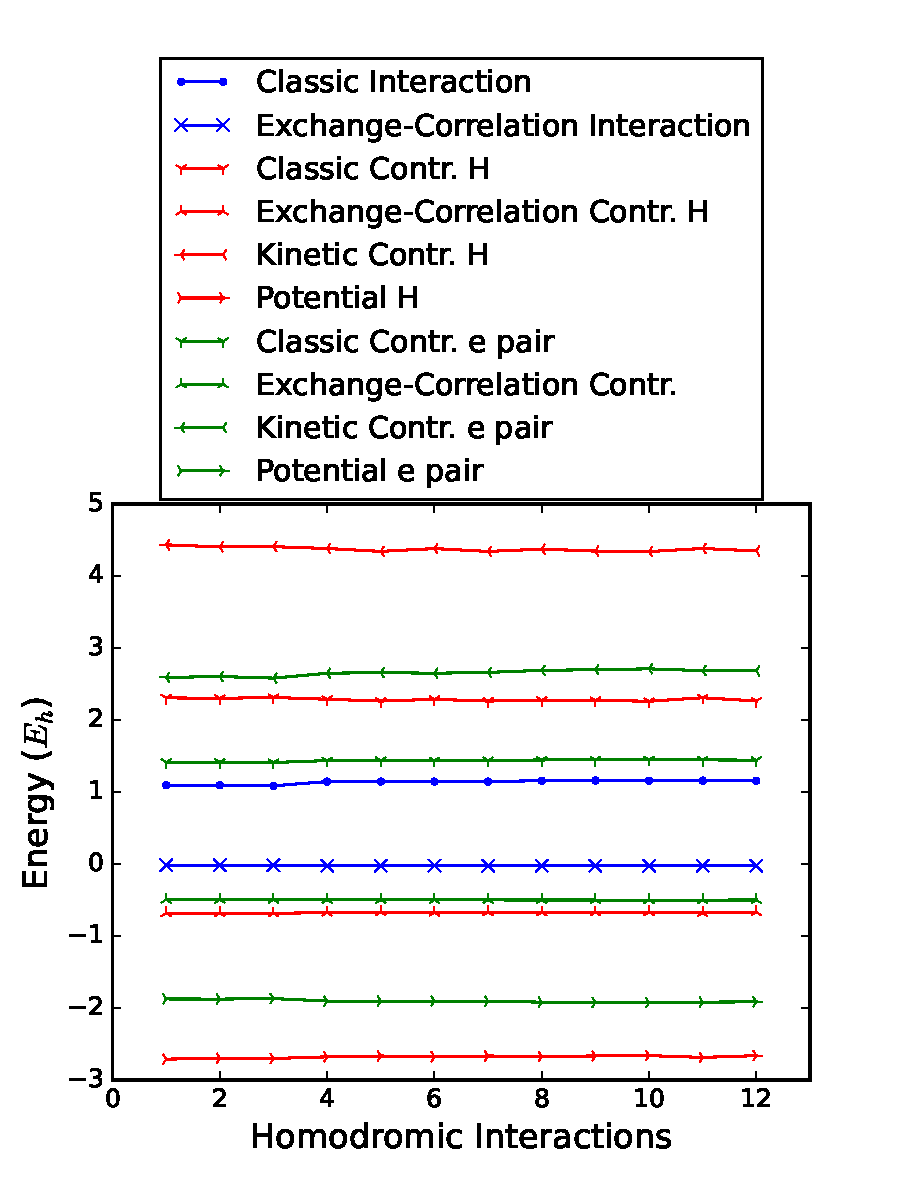
\includegraphics[width=0.5\textwidth]{4/plots/promelf/homodromic1.pdf}
    \caption{Contributions for HB in Homodromic Cases.}
    \label{homodromic}
\end{wrapfigure}

As was mentioned before, the homodromic clusters has a particular trend. The
size does not really affect the ratio between the different energy
contributions to the HB interaction (see Figure \ref{homodromic}), \textit{i.
e.}, what does not change is the proportion between the different contributions
to the interaction energy.

In \citet{Castor2020} work is shown that the strength of the HBs is related to
the coordination between water molecules, paying attention to their roles as
acceptors or donors. In our work, we have tried to reproduce these trends.

For the water clusters analyzed in this work, we have 6 types of the 10 that
are reported in \citenum{Castor2020}. The 6 types are plotted in the Figure
\ref{typesHB}.

Comparing the data obtained in this work and the reported in
\citenum{Castor2020} we cannot claim that we predict exactly the same trend,
since the dispersion data is too big to say whether it is the same trend or
not. This dispersion could be due to three things, $i$) we do not have enough
interactions to have a good statistic analysis, $ii$) the \citenum{Castor2020}
work takes into account how the water molecules are affected since are not in
theirs equilibrium geometry when their are not interacting with another
chemical entity, that by the deformation energy, and $iii$) the topology for
the ELF is more elaborated that the $\rho$ topology (used in the
\citenum{Castor2020} work) giving troubles for the computational integrals.

In particular, this last reason will be a future perspective, as computational
problems around water clusters with {\sc{Promelf}} program arise once again
while doing the topology calculations with $\rho$.

\newpage

The different types of HB as function of connectivity are shown in the Figure
\ref{typesHB}, and in the Figure \ref{escala2020} are the values obtained in
this work and the computed in \citenum{Castor2020} are compared.  We can see
how the types 8, 9, 10 have the same trend in both works. However, the type 4
in the work \citenum{Castor2020} has basically the same value compared with the
type 5, where in this work we have a significant difference and with the
opposite trend that in \citenum{Castor2020}, whereas the error bars are enough
big to aim that the two topology perspectives predict different conclusions.

\begin{figure}
  \begin{minipage}[t]{0.49\textwidth}
    \centering
    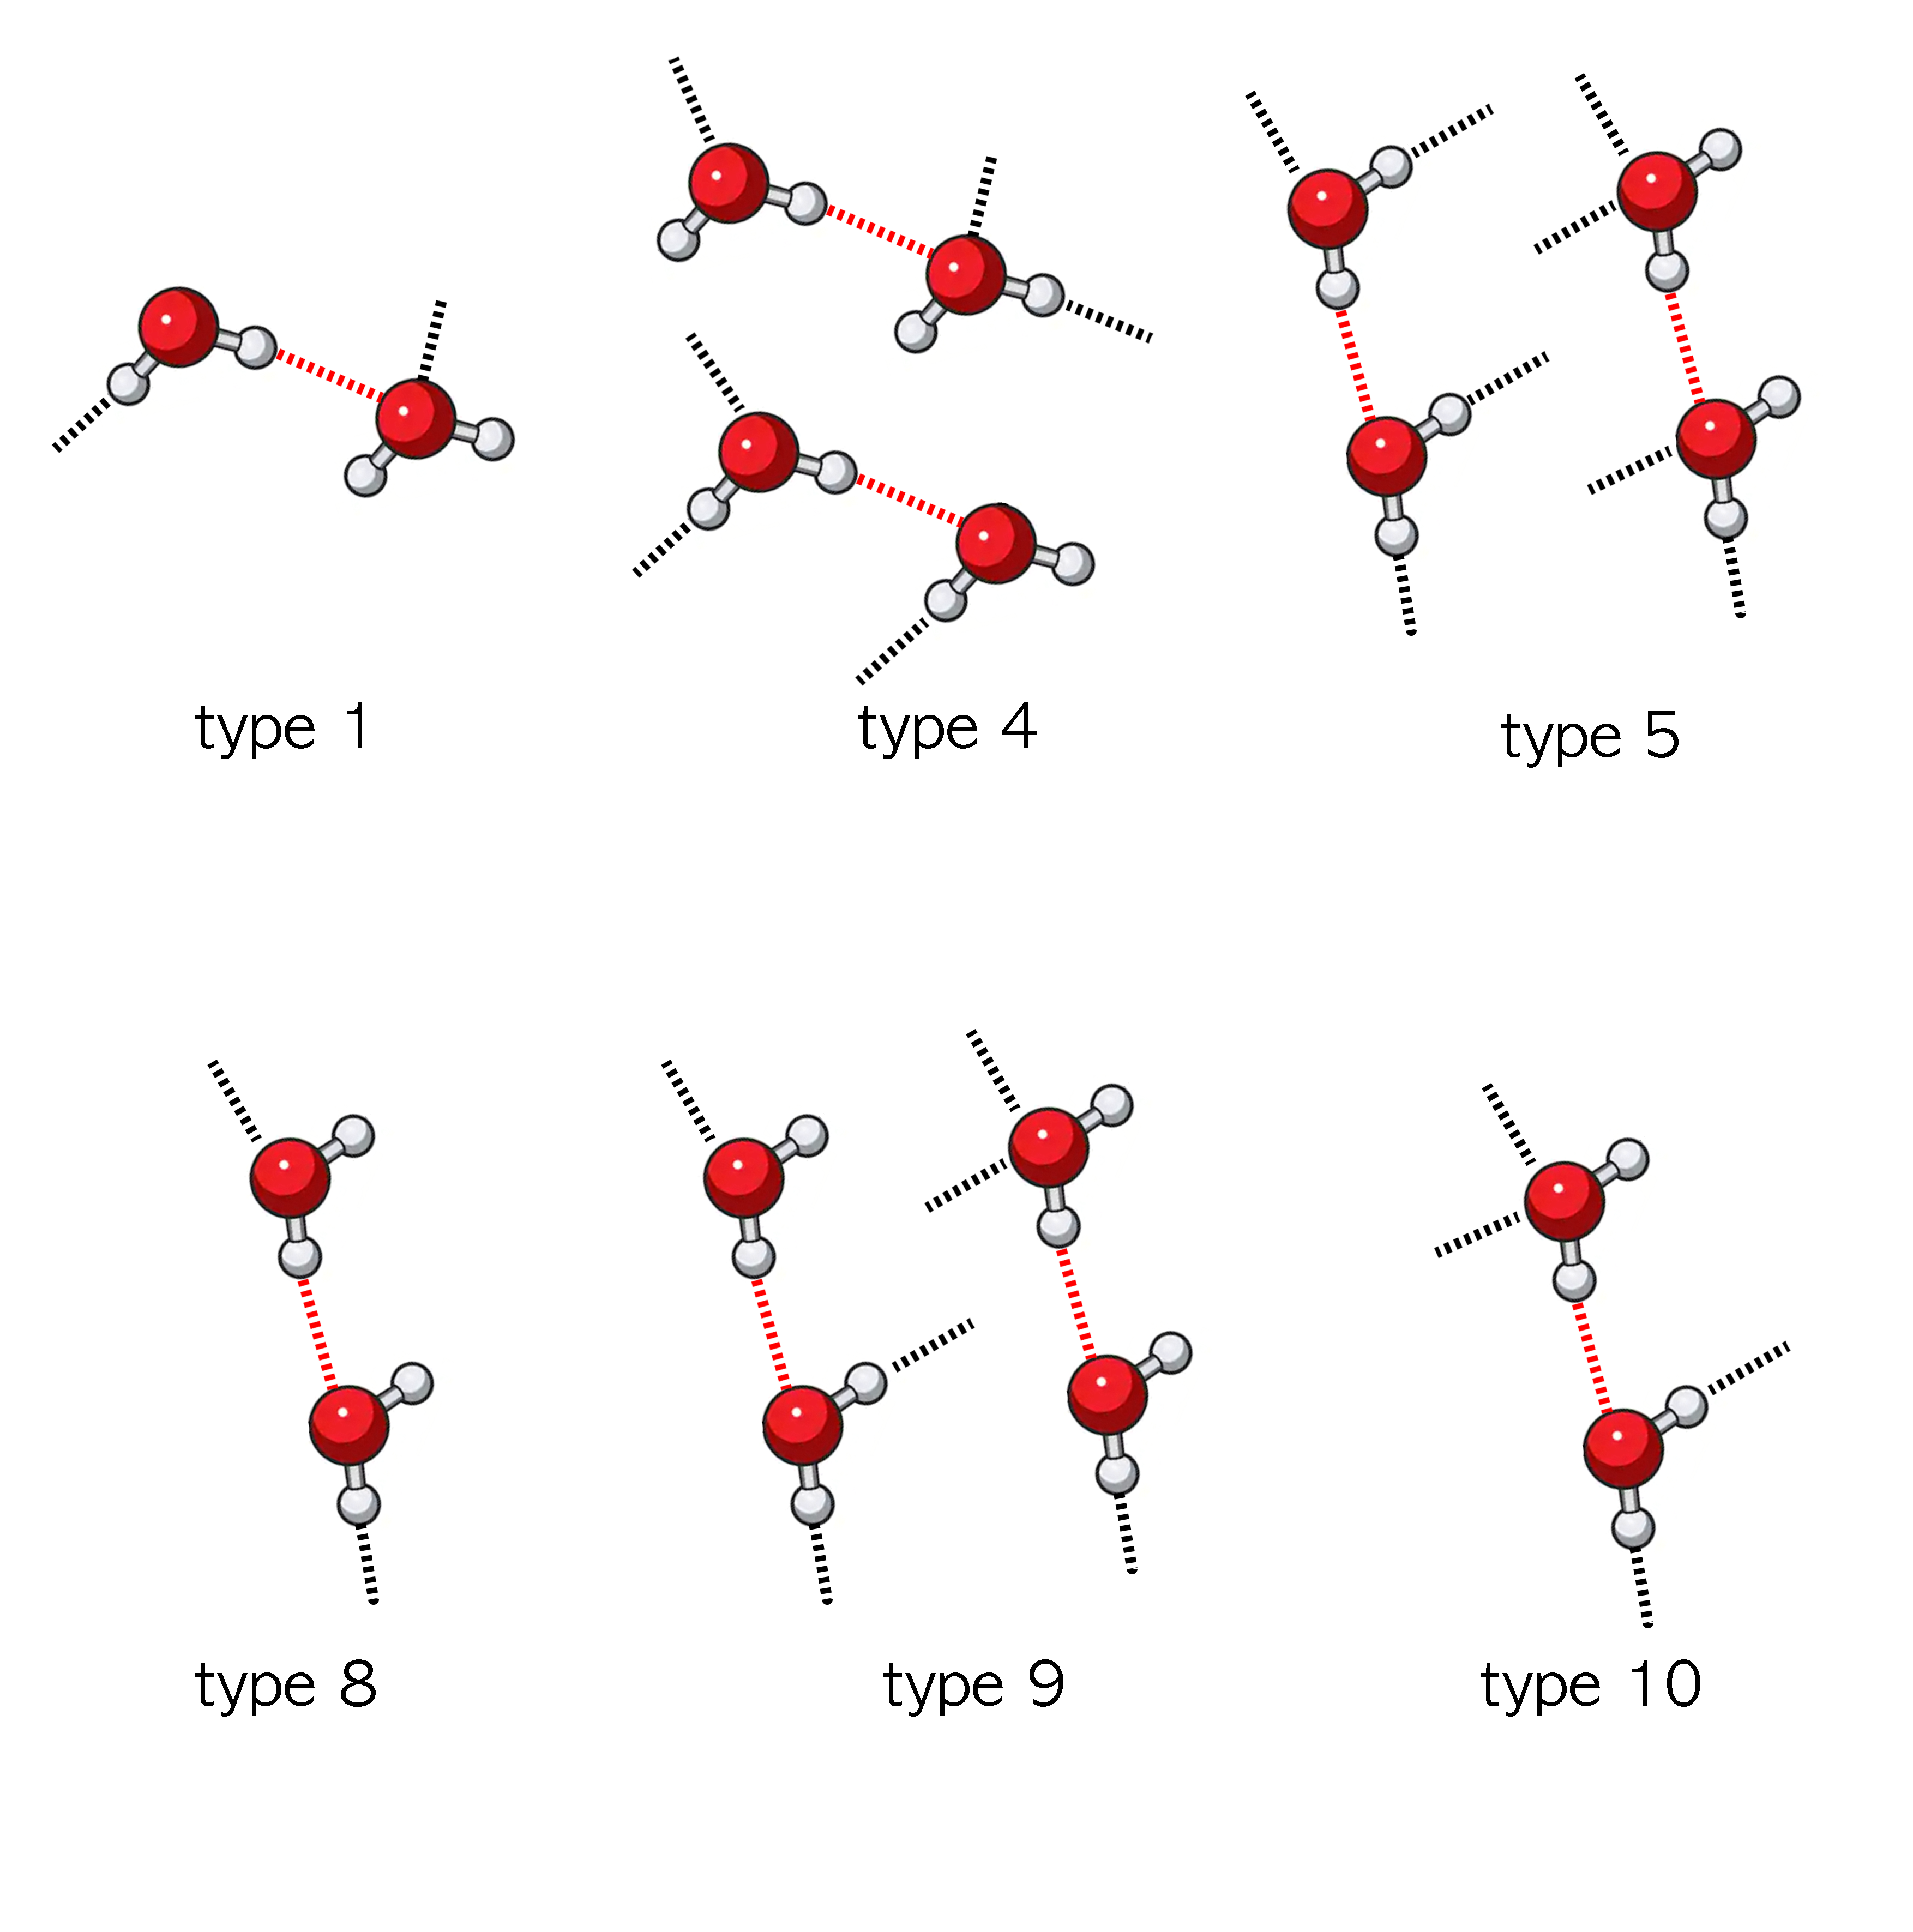
\includegraphics[width=\textwidth]{4/plots/dibujitos/awitas.png}
    \caption{Types of HB in the analyzed water clusters.}
    \label{typesHB}
  \end{minipage}%
  \hfill
  \begin{minipage}[t]{0.49\textwidth}
    \centering
    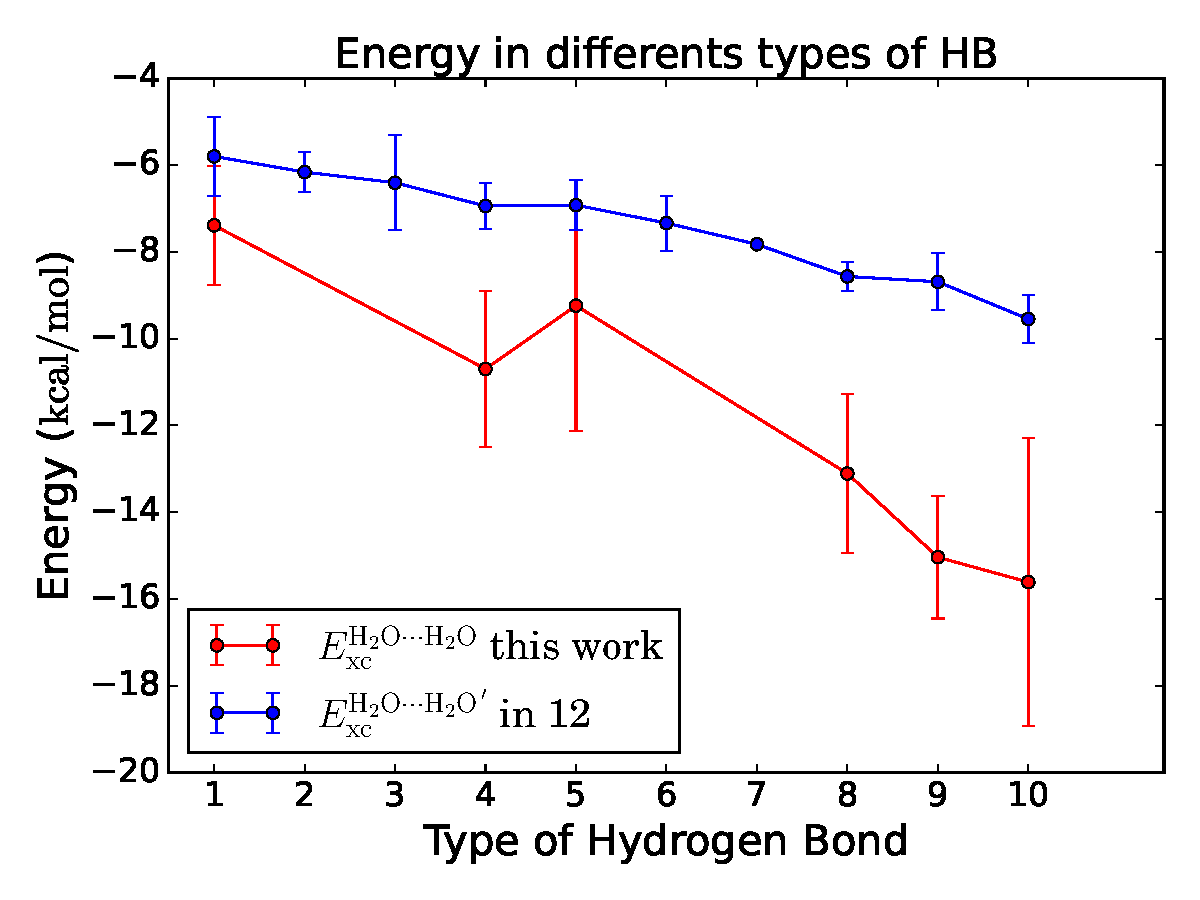
\includegraphics[width=\textwidth]{4/plots/promelf/types.pdf}
    \caption{Comparison between the scale shown in \citenum{Castor2020} and this work.}
    \label{escala2020}
  \end{minipage}%
\end{figure}
